% Este template foi desenvolvido por Prof. Luis Fernando de Oliveira IF/UERJ
% e adaptado para uso na UNILA pelo Prof. Joylan N. Maciel em 07/06/2023
% Todos os crédito são do Prof. Luis Fernando de Oliveira IF/UERJ
% Este template/modelo serve para fazer TCC, Dissertação ou Tese de Doutorado

\documentclass[a4paper,12pt,oneside,onecolumn,final,fleqn]{repUERJ}
% Pacotes fundamentais 
\usepackage[english,brazil]{babel}  % adequação para o português Brasil
\usepackage[utf8]{inputenc} % Determina a codificação utilizada
                            % (conversão automática dos acentos)
\usepackage{makeidx}        % Cria o índice
\usepackage{hyperref}       % Controla a formação do índice
\usepackage{indentfirst}    % Endenta o primeiro paragrafo de
                            % cada seção.
\usepackage{graphicx}       % Inclusão de gráficos
\usepackage{subfig}
\usepackage{amsmath}        % pacote matemático
\usepackage{bm}             % pacote de fontes matematicas
\usepackage{lscape}         % pacote para colocar páginas em landscape
\usepackage{array}
\usepackage{ragged2e}
\usepackage{wrapfig}
\usepackage[table,xcdraw]{xcolor}
\usepackage{placeins}


% ---
% Pacote auxiliar para as normas da UERJ
% ---
\usepackage[frame=no,font=default]{repUERJformat}
\usepackage[line=yes]{repUERJpseudocode}
% ---
% Pacotes de citacoes
% ---
\usepackage[alf,abnt-repeated-author-omit=no]{abntex2cite}


\selectlanguage{brazil} % setando o idioma global para português



% ********************************************************************
% ********************************************************************
% Área Reservada para incluir os novos comandos
% ********************************************************************
% ********************************************************************

% Comandos de comentários
\definecolor{green}{rgb}{0.1, 0.4, 0.1}
\newcommand\red[1]{{\color{red}#1}}
\newcommand\sred[1]{{\color{red}\uline{#1}}}
\newcommand\blue[1]{{\color{blue}#1}}
\newcommand\sblue[1]{{\color{blue}\uline{#1}}}
\newcommand\green[1]{{\color{green}#1}}
\newcommand\sgreen[1]{{\color{green}\uline{#1}}}
\newcommand\orange[1]{{\color{orange}#1}}
\newcommand\sorange[1]{{\color{orange}\uline{#1}}}
%o comando \sout funciona para riscar o texto

% % Abaixo tem-se alguns exemplos de definição de comandos

% \newcommand\dd{\mathrm{d}} % d de derivada
% \newcommand\DD{\mathrm{D}} % D de derivada
% \newcommand\ee{\mathrm{e}} % número natural: e
% \newcommand\ii{\mathrm{i}} % número complexo: i

% \newcommand\Vol{\mathcal{V}} % Simbolo de volume

% \newcommand\Vector[1]{\mbox{\boldmath$#1$}} % comando para colocar vetores
% \newcommand\Tensor[1]{\mbox{\boldmath$\mathrm{#1}$}} % comando para colocar tensores/matrizes

% %Alguns exemplos de definição de vetores, tensores e matrizes
% \newcommand\vvec{\Vector{v}} % vetor
% \newcommand\Tten{\Tensor{T}} % Tensor
% \newcommand\Mmat{\Tensor{M}} % Matriz

% % Alguns parâmetros adimensionais
% \newcommand\Bi{\mathrm{Bi}} % Número de Biot
% \newcommand\Rey{\mathrm{Re}} % Número de Reynolds
% \newcommand\Ma{\mathrm{Ma}} % Número de Mach
% \newcommand\Pe{\mathrm{Pe}} % Número de Péclet

% \newcommand\Dh{D_H} % Diâmetro hidráulico

% % Alguns índices máximos 
% \newcommand\nmax{n_{\text{max}}}
% \newcommand\mmax{m_{\text{max}}}
% \newcommand\imax{i_{\text{max}}}
% \newcommand\jmax{j_{\text{max}}}








% ********************************************************************
% ********************************************************************
% Informações de autoria e institucionais
% ********************************************************************
% ********************************************************************

%---------------------------------------------------------------------
% Imagens pretextuais (precisam estar no mesmo diretório deste arquivo .tex)
%---------------------------------------------------------------------

\logo{Figuras/logo_UNILA.jpg}
% \marcadagua{marcadagua_uerj_cinza.png}{1}{160}{255}

%---------------------------------------------------------------------
% Informações da instituição
%---------------------------------------------------------------------
\instituicao{Instituto Latino Americano de Ciências da Vida e da Natureza (ILACVN)}  %Instituto
            {Biotecnologia}  %Curso
            {} %Unidade (DEIXAR EM BRANCO)
            {} %Departamento (DEIXAR EM BRANCO)

%---------------------------------------------------------------------
% Informações da autoria do documento
%---------------------------------------------------------------------

\autor{Samuel}
      {Chagas de Assis}
      {S.C.A.} % iniciais do nome

\titulo{Análise genômica das variantes de SARS-CoV-2 detectadas em Foz do Iguaçu - Paraná/BR e o impacto das mutações \textit{missense} nas vias dependentes de HLA-B } %Título do trabalho acadêmico em português
%\title{ProjetoTCC} %Título do trabalho acadêmico em inglês



\orientador{Profa.} %cargo, ex.: Prof., Profa., Eng. , etc...
		   {Maria Cláudia}{Gross, Ph.D.} %Nome sobrenome com a titulação ao final. Exemplo: D.Sc., Ph.D., M.Sc., B.Sc., etc.
           {Universidade Federal da Integração Latino Americana (UNILA) - ILACVN} % Instituição e Departamento ou PPG


%Opcional, Comente as linhas de coorientador caso não tenha
%\coorientador{Prof.}  %cargo, ex.: Prof., Profa., Eng. , etc...
%           {Astrogildo}{Silva, Me.}  %Nome sobrenome com a titulação ao final. Exemplo: D.Sc., Ph.D., M.Sc., B.Sc., etc.
%           {Universidade Federal da Integração Latino Americana (UNILA) - ILACVN} % Departamento ou PPG e Instituição 

%---------------------------------------------------------------------
% Grau pretendido (Doutor, Mestre, Bacharel, Licenciado) e Curso
%---------------------------------------------------------------------
%Descomente as sua opções

%\newcommand\artigo{à}%Projeto de graduação
% \newcommand\artigo{ao}%Pós Graduação


\grau{Graduação}
%\grau{Mestre} 
%\grau{Doutor}


\curso{Bacharelado em Biotecnologia}
\newcommand\grauTitulo{Bacharel em Biotecnologia}  


%\areadeconcentracao{} %Projeto de Graduação
%\areadeconcentracao{Área de Concentração} %Pós Graduação
%\areadeconcentracao{Mecânica dos Sólidos} %Pós Graduação



%---------------------------------------------------------------------
% Informações adicionais (local, data e paginas)
%---------------------------------------------------------------------

\local{Foz do Igua\c{c}u} 
\data{10}{Novembro}{2024} % Exemplo: \data{21}{Março}{2016}

% ********************************************************************
% ********************************************************************
% Configurações de aparência do PDF final
% ********************************************************************
% ********************************************************************

% alterando o aspecto da cor azul
\definecolor{blue}{RGB}{41,5,195}
%\definecolor{apricot}{RGB}{251,206,177}

% informações do PDF
\hypersetup{
  unicode=false,
  pdftitle={\UERJtitulo},
  pdfauthor={\UERJautor},
  pdfsubject={\UERJpreambulo},
  pdfkeywords={PALAVRAS}{CHAVES}{\chaveA}{\chaveB}{\chaveC}{\chaveD},
  pdfproducer={\packagename}, % producer of the document
  pdfcreator={\UERJautor},
  colorlinks=true,            % false: boxed links; true: colored links
  linkcolor=black,            % color of internal links blue
  citecolor=black,            % color of links to bibliography blue
  filecolor=black,            % color of file links magenta
  urlcolor=black,
  bookmarksdepth=4
  %backref=true,
  %pagebackref=true,
  %bookmarks=true,
}

% ********************************************************************
% ********************************************************************
% Início do documento
% ********************************************************************
% ********************************************************************
% ---
% compila o índice; se não for usar, comentar
% ---
\makeindex
% ********************************************************************
% ********************************************************************
\begin{document}
% ----------------------------------------------------------
%% ELEMENTOS PRE-TEXTUAIS
% ----------------------------------------------------------
\frontmatter
% ----------------------------------------------------------
% Capa e a folha de rosto
% ----------------------------------------------------------
\capa
\folhaderosto
% ----------------------------------------------------------
% Inserir a ficha catalográfica
% ----------------------------------------------------------
% ---
% A biblioteca deverá providenciar a ficha catalográfica. Salve a ficha no
% formato PDF. Use o nome do arquivo PDF como argumento do comando. 
% Exemplo: ficha catalográfica é o arquivo 'Ficha.pdf' na pasta "B.PreTextual"
%     \fichacatalografica{B.PreTextual/Ficha.pdf}
%
% Enquanto não possuir a ficha catalográfica, use o comando sem argumentos.
% ---
%\fichacatalografica{B.PreTextual/Ficha.pdf}



% ----------------------------------------------------------
% Folha de aprovação
% ----------------------------------------------------------

%Após obter a assinatura dos membros da banca, comente as linhas a baixos e insira o pdf com as assinaturas na pasta "B.PreTextual"


% Ajustar o espaço entre as assinaturas abaixo
\newcommand{\spc}{0.25cm}

\begin{folhadeaprovacao}
	\vspace{\spc} % Espaço entre assinaturas
	\assinatura{Prof. Kelvinson Fernandes Viana, Ph.D.}{UNILA}
	\vspace{\spc} % Espaço entre assinaturas
        \assinatura{Profa. Maria Leandra Terencio, Ph.D.}{UNILA}
	\vspace{\spc} % Espaço entre assinaturas

\end{folhadeaprovacao}


% Após colocar o pdf com as assinaturas na pasta "B.PreTextual", comente todo o ambiente "folhadeaprovacao" acima, descomente a linha abaixo e insira o nome correto do arquivo pdf:
%\includepdf[pages=1]{B.PreTextual/ficha.pdf} %exemplo


% ----------------------------------------------------------
% Dedicatória
\pretextualchapter{Dedicatória}
\vfill
Dedico este trabalho à minha família, especialmente, ao Tio Cid (\textit{in memorian}), uma das muitas vidas negligenciadas durante a pandemia de COVID-19.  






% ----------------------------------------------------------
% Agradecimentos
\pretextualchapter{Agradecimentos}

\begin{justify}

\hspace{12 mm}Minha trajetória acadêmica é um reflexo dos incontáveis esforços que meu pai, Caetano, e minha mãe, Márcia, realizaram para me propiciar a oportunidade de estudar. A eles agradeço as oportunidades, as motivações e os ensinamentos que foram cultivados anos atrás pela Vó Clara, Vô Onélio, Vó Gleci e o Vô Nelson. 

O interesse pela ciência e pesquisa  que foi cultivada por meio de discussões e ensinamentos compartilhados com minha irmã, Caroline, a quem agradeço por ser minha maior inspiração pessoal e profissional.

A motivação diária para conclusão deste trabalho é fruto dos momentos inspiradores e as conversas de conforto com minha namorada Alexia, a quem agradeço pelo amor e o companheirismo de sempre. 

Transformar esses anos de graduação com momentos memoráveis e fazer da minha casa, em Foz do Iguaçu, um verdadeiro lar foi devido àqueles com quem compartilhei cada instante. Ao Felipe (Felps), Anderson (Dylon), Michelli, Maria, Rosane, Matheus, Giulio e Andressa, agradeço por serem tão especiais para mim e pelos cafézinhos, a parceria, o carinho e a paciência.

Por me proporcionar a oportunidade de acessar um conhecimento para além das fronteiras e serem grandes amigos, agradeço ao Eric, Julio, Lucas, Ângelo e Bernie pelo conhecimento e os momentos compartilhados. 

A possibilidade de contribuir cientificamente no Laboratório de Pesquisa em Ciências Médicas (LPCM) e abrir portas para outras oportunidades foi graças a orientação da Profa. Dra. Maria Claudia Gross, a quem agradeço pelas conversas e orientação.

A Profa. Dra. Maria Leandra Terencio e Prof. Dr. Carlos Henrique Schneider agradeço o suporte e atenção nas etapas de experimentais do meu projeto de iniciação científica, o qual resultou nos dados experimentais utilizados nensse trabalho. 

Aos participantes de cada projeto que acreditaram nas ideias mais (in)consequentes possíveis durante a graduação, agradeço pela parceria e dedicação, especialmente àqueles que confiaram no potencial do Centro Acadêmico de Biotecnologia - UNILA e do Grupo de Biologia Sintética SynFronteras.

Ao Corpo Docente do Curso de Biotecnologia, agradeço a dedicação diária em enfrentar os desafios, de um curso novo em uma universidade nova, no suporte para transformação e formação de novos profissionais. 

Agradeço a UNILA pela educação pública, gratuita e de qualidade, além de ressignificar para mim a integração latino-americana no desenvolvimento socioeconômico, cultural e político do povo.


\end{justify}



% ----------------------------------------------------------
% Epigrafe (opcional)
\pretextualchapter{}
\vfill
\begin{flushright}
	\textit{Es América Latina, la región de las venas abiertas. [...] \\
        La causa nacional latinoamericana es, ante todo, una causa social.}\\
	\textbf{\textit{Eduardo Galeano \\ Las venas abiertas de América Latina, 1978, p. 14 e 281.}}
\end{flushright}










% ----------------------------------------------------------
%% RESUMO
% se não for usar a quarta palavra chave, deixar o campo vazio: {}
\palavraschaves{COVID-19}
{variações alélicas}
{complexo de histocompatibilidade}
{sequenciamento}



\pretextualchapter{Resumo}


\begin{justifying}

A vigilância genômica do SARS-CoV-2 tem sido fundamental para monitorar o surgimento de mutações e compreender suas implicações na severidade e disseminação do vírus, auxiliando na previsão de impactos na eficácia da vacinação e na resposta imune populacional. Neste estudo computacional, mapeamos as variantes de SARS-CoV-2 circulantes em Foz do Iguaçu, Paraná, Brasil, de 2020 a 2022. Focamos na identificação de mutações \textit{missense}, que alteram a sequência de aminoácidos das proteínas virais, e avaliamos seu efeito na apresentação de epítopos, com ênfase nos alelos HLA-B da população local. Os resultados indicaram que epítopos associados aos alelos B*07:02 e B*27:05 apresentaram maior perda de ligação devido a mutações, e que a dinâmica de algumas variantes pode demonstrar a exportação de variantes ao Paraguai. Embora não tenha sido observada uma correlação direta entre o perfil alélico de pacientes internados em UTI e a circulação de mutações específicas, o estudo revelou a dinâmica mutacional do SARS-CoV-2 ao longo do tempo em Foz do Iguaçu durante a pandemia. Dessa forma, a pesquisa identificou mutações que potencialmente impactaram a disseminação do vírus e ofereceu um panorama das variantes circulantes, contribuindo para futuras estratégias de vigilância epidemiológica na região fronteiriça.

\end{justifying}

\imprimirchaves % linha em branco antes




% ----------------------------------------------------------
% Abstract
\begin{otherlanguage}{english}
\keywords{COVID-19}
{allelic variance}
{major histocompatibility complex}
{sequencing}

\pretextualchapter{Abstract}


% O resumo em inglês deve ser organizado em apenas um parágrafo mesmo.

\begin{justifying}

Genomic surveillance of SARS-CoV-2 has been essential for monitoring emerging mutations and understanding their implications for viral severity and spread, aiding in predicting impacts on vaccine efficacy and the population's immune response. In this computational study, we mapped SARS-CoV-2 variants circulating in Foz do Iguaçu, Paraná, Brazil, from 2020 to 2022. We focused on identifying missense mutations, which change the viral protein amino acid sequence in an unique position, and assessed their effect on epitope presentationfor HLA-B alleles. The results indicated that epitopes associated with the B*07:02 and B*27:05 alleles showed greater binding loss due to mutations, and that the emergence of certain variants may be related to the city’s proximity to Paraguay. Although no direct correlation was found between the allelic profile of ICU-admitted patients and the circulation of specific mutations, the study revealed SARS-CoV-2's mutational dynamics over time in Foz do Iguaçu during the pandemic. Thus, this research identified mutations potentially impacting viral spread and provided an overview of circulating variants, contributing to future epidemiological surveillance strategies.

\end{justifying}

\printkeys % linha em branco antes


\end{otherlanguage}

% Abstract
%\begin{otherlanguage}{spanish}
%\pretextualchapter{Resumen}
\reference % linha em branco depois

% O resumo em espanhol deve ser organizado em apenas um parágrafo mesmo.


La vigilancia genómica de SARS-CoV-2 ha sido fundamental para monitorear la aparición de mutaciones y entender sus implicaciones en la gravedad y propagación del virus, ayudando a prever los impactos en la eficacia de la vacunación y en la respuesta inmune de la población. En este estudio, mapeamos las variantes de SARS-CoV-2 circulantes en Foz do Iguaçu, Paraná, Brasil, entre 2020 y 2022. Nos centramos en identificar mutaciones missense, que alteran la secuencia de aminoácidos de las proteínas virales, y evaluamos su efecto en la presentación de epítopos, especialmente para los alelos HLA-B en la población local. Los resultados indicaron que los epítopos asociados con los alelos B07:02 y B27:05 presentaron una mayor pérdida de unión debido a mutaciones, y que la aparición de ciertas variantes puede estar relacionada con la proximidad de la ciudad a Paraguay. Aunque no se encontró una correlación directa entre el perfil alélico de pacientes ingresados en la UCI y la circulación de mutaciones específicas, el estudio reveló la dinámica mutacional del SARS-CoV-2 a lo largo del tiempo en Foz do Iguaçu durante la pandemia. Así, esta investigación identificó mutaciones que potencialmente afectaron la propagación del virus y proporcionó una visión general de las variantes circulantes, contribuyendo a futuras estrategias de vigilancia epidemiológica.

\noindent Palavras-clave: SARS-CoV-2; genómica; variantes; Foz do Iguaçu


%\end{otherlanguage}


% ----------------------------------------------------------
% Listas de ilustrações e tabelas
% ----------------------------------------------------------
\listadefiguras
\listadetabelas
% ----------------------------------------------------------
% Outras listas
% ----------------------------------------------------------
%\listadealgoritmos


% ----------------------------------------------------------
% Lista de abreviaturas e siglas
\pretextualchapter{Lista de abreviaturas e siglas}
% ---
\abreviatura{ACE2}{Angiotensin-converting enzyme 2 (Enzima Conversora de Angiotensina 2)}
\abreviatura{FC}{Fold change (Razão da expressão relativa)}
\abreviatura{FCS}{Furin cleavage site (Sítio de Clivagem da Furina)}
\abreviatura{GISAID}{Global Initiative on Sharing All Influenza Data}
\abreviatura{HLA-B}{Human Leukocyte Antigen Class I - B (Antígeno Leucocitário Humano Classe I - B)}
\abreviatura{HMPGL}{Hospital Municipal Padre Germano Lauck}
\abreviatura{MHC}{Major Histocompatibility Complex (Complexo Principal de Histocompatibilidade)}
\abreviatura{RBD}{Receptor Binding Domain (Domínio de Ligação ao Receptor)}
\abreviatura{ORF}{Open Reading Frame}
\abreviatura{VOC}{Variant of Concern (Variante de Preocupação)}
\abreviatura{VOI}{Variant of Interest (Variante de Interesse)}












% ----------------------------------------------------------
% Lista de simbolos
%\include{B.PreTextual/08.ListaSimbolos}

% ----------------------------------------------------------
% Sumario
\sumario

% ----------------------------------------------------------
%% ELEMENTOS TEXTUAIS
% ----------------------------------------------------------
\mainmatter



%=====================================================================
 % Na introdução deve-se utilizar \chapter* e \section* 
\chapter{Introdução}
%=====================================================================
\begin{justify}

\hspace{12 mm}A vigilância genômica das variantes circulantes de SARS-CoV-2 permitiu o acompanhamento do surgimento de mutações que pudessem gerar impactos na severidade e circulação do vírus. No entanto, mutações neutras ou moderadamente deletérias foram observadas em grande parte da amostragem presente no banco de dados \textit{Global Initiative on Sharing All Influenza Data} (GISAID). Esse fator se deve à tendência de mutações com grande efeito fenotípico serem minoria comparado às toleradas modificações de aminoácidos de baixo- ou sem-efeito \cite{Harvey:2021}.

Porém, essa pequena minoria de modificações pode contribuir para o aumento do \textit{fitness} e conferir determinadas vantagens em diferentes ciclos virais, como: patogenicidade, infectividade, transmissibilidade e/ou antigenicidade. Nesse sentido, ao longo da pandemia surgiram evidências que alterações fenotípicas das variantes virais estavam diretamente relacionadas com alterações no mecanismo de resposta (neutralização por anticorpos) e reconhecimento (ligação pelos complexos de apresentação de antígeno) do sistema imune \cite{Harvey:2021, Pontarotti:2022}.

Portanto, esforços foram concentrados em compreender essas diferenças de resposta imune para avaliar o comportamento evolutivo viral, como também, compreender as regiões e marcadores que podem afetar a eficácia de uma vacinação em massa. Em termos de reconhecimento do sistema imune, diferentes trabalhos mapearam epítopos de SARS-CoV-2, a partir da linhagem de origem em Wuhan, China,  que são potencialmente reconhecidos por células T \cite{Grifoni:2020, Kiyotani:2020}.

Essa diversificação do quadro de apresentação de antígenos baseado nas informações mutacionais foi explorada por \citeonline{Hamelin:2022}, onde se avaliou o impacto das mutações prevalentes, detectadas na vigilância genômica global de SARS-CoV-2, demonstrando que a identificação de determinadas mutações e grupos alélicos que apresentam influência na resposta imune, baseada na apresentação de epítopos, se torna um indicador de que a monitoramento genômico viral e a identificação do perfil HLA populacional podem convergir para avaliar o quadro de incidência da doença em determinada região e no desenvolvimento de novas vacinas.

Em relação a regiões de fronteira, esses indicadores se tornam mais difíceis de medir e avaliar. O trânsito comercial e urbano podem gerar perturbações em relação a vigilância epidemiológica de cada país, devido a circulação de  novas variantes e a diversificação genômica presente na população de fronteira. Portanto, o presente trabalho busca mapear as variantes que potencialmente circularam no município de Foz do Iguaçu - Paraná/BR e a influência das mutações \textit{missense} - uma mutação pontual que codifica um aminoácido não-sinônimo -  na apresentação de epítopos em relação ao perfil alélico de HLA-B da região.

\end{justify}
\chapter{Revisão Bibliográfica}

\begin{justify}

\section{O Complexo Principal de Histocompatibilidade e o Sistema de Antígeno
Leucocitário Humano (HLA)}

O Complexo Maior de Histocompatibilidade (\textit{Major Histocompatibility Complex} - MHC, em inglês) exerce um papel fundamental no sistema imune, responsáveis pela apresentação de peptídeos na superfície celular para reconhecimento das células T \cite{Wieczorek:2017}. A versão humana do MHC , chamado de sistema HLA (\textit{Human Leukocyte Antigen}, em inglês) é codificado a partir do cromossomo 6 e estima-se que apresenta cerca de 40 diferentes genes de HLA, extremamente polimórficos, distribuídos em três classes.  No entanto, apenas duas classes, I e II, estão envolvidas com a resposta imune e possuem diferentes funções e estruturas \cite{Klein:2000}. 

Os genes da Classe I são consideravelmente expressos em células somáticas e dependem do tipo de tecido, já a Classe II está presente nas células do sistema imune incluindo células B, células T ativadas, macrófagos, células dendríticas, etc \cite{Klein:2000, Siegrist:2018}. As Classes I e II também se dividem na localização celular e para entender seu funcionamento é necessário compreender a dinâmica celular no processamento de peptídeos intra- e extracelulares. No citosol, proteínas defeituosas, indesejadas ou desgastadas são processadas pelo proteossoma a partir do reconhecimento da ubiquitina. Esse processamento gera peptídeos que são transportados, com auxílio da classe de Transportadores Associados com o Processamento de Antígenos (TAP, sigla em inglês),  para o retículo endoplasmático e dependendo de sua afinidade de ligação, são reconhecidos pelo MHC Classe I e exportados por meio do Complexo de Golgi até a superfície extracelular (Figura \ref{fig:fig1}A) \cite{Klein:2000}. 

Por outro lado, as proteínas adquiridas do espaçamento extracelular são processadas de maneira diferente. A partir da endocitose (ou fagocitose), as proteínas extracelulares são processadas por meio do mecanismo lisossomal com proteínas proteolíticas para formação de endossomos e reciclagem de aminoácidos. Durante o processamento, o MHC Classe II reconhece os peptídeos pré-processados baseados na afinidade de ligação e são exportados para superfície extracelular (Figura \ref{fig:fig1}B) \cite{Klein:2000}.

Apesar de haver uma diferença funcional e de localização entre as duas classes, seu funcionamento não é restrito às suas atribuições previamente descritas. Em alguns casos, peptídeos extracelulares são processados pela Classe I e peptídeos intracelulares são processados pela Classe II \cite{Klein:2000}.

\begin{wrapfigure}{c}{\textwidth}
    \centering
    \caption{\justifying Processamento dos antígenos para apresentação ao sistema imune. (A) Principal via de geração dos peptídeos para apresentação pelas moléculas HLA Classe I; (B) e Classe II. }
    \includegraphics[width=0.7\textwidth]{Figuras/fig1.png}
    \label{fig:fig1}
    \begin{minipage}{0.7\textwidth} % Adjust width as needed
        \centering
        \footnotesize Fonte: \citeonline{Klein:2000}
    \end{minipage}

\end{wrapfigure}

\begin{wrapfigure}{c}{0pt}
\end{wrapfigure}

\section{Estrutura  e Apresentação à Células T}

As estruturas da Classe I e II são compostas por dois domínios, com uma única cadeia-a pesada (Classe I) ou com duas cadeias, cadeia-$\alpha$ e cadeia-$\beta$ (Classe II). Os dois domínios formam uma base folha-$\beta$ e duas $\alpha$-hélices no topo, onde são acomodados os peptídeos. Cada cadeia apresenta um domínio de imunoglobulina, enquanto o MHC Classe I é associado a uma cadeia leve de $\beta$-2 microglobulina ($\beta$2m). Por fim, hélices transmembrana ancoram os complexos na membrana \cite{Wieczorek:2017}.

Os genes que compreendem as Classes I e II apresentam alto grau de polimorfismo (os mais conhecidos são: Classe I: HLA-A, -B, -C; Classe II: HLA-DR, -DP, -DQ), os quais possuem uma variação alélica que afeta a ligação de peptídeos nos sulcos de ligação e modulam a seleção de peptídeos apresentados na superfície celular pelo MHC. No sulco de ligação, a estrutura helicoidal se liga aos peptídeos de acordo com a (i) formação de ligações de hidrogênio entre as estruturas do MHC e o peptídeo e a (ii) ocupação de pequenos espaços que ancoram resíduos da cadeia lateral peptídica \cite{Wieczorek:2017}. Apenas alguns desses pequenos espaços já podem determinar a especificidade de cada peptídeo em se ligar ao complexo e geralmente é definido pela conformação dos diferentes alelos \cite{Klein:2000}.

Essa interação das cadeias laterais de cada peptídeo depende da geometria, distribuição de carga e hidrofobicidade na ligação ao sulco. No entanto, a predição de afinidade nessa interação MHC-antígeno não depende somente das características moleculares, como o tamanho (8-12 resíduos para Classe I e 13-25 resíduos para Classe II) ou composição das cadeias laterais,  se não das conformações transitórias e energéticas das estruturas do MHC durante suas flutuações de equilíbrio da estrutura molecular. Por isso, o carregamento do MHC é influenciado por diferentes fatores, como disponibilidade de antígenos, atividade das proteases, disponibilidade de chaperonas e interação com proteínas auxiliares, como a Tapasina (Classe I) e HLA-DM (Classe II) \cite{Wieczorek:2017}.

A partir da ligação, o MHC é transportado até a superfície celular para apresentação do antígeno para células T. Na região dos linfonodos, as células T CD4+ reconhecem os antígenos apresentados pela Classe II, enquanto as células T CD8+ reconhecem o complexo MHC-peptídeos formados pela Classe I. O reconhecimento dos peptídeos, geralmente, não são o suficiente para ativação das células T, as quais permanecem anérgicas ou se tornam tolerantes na falta de um estímulo secundário \cite{Siegrist:2018}. 

\section{Estrutura e Processo de Infecção de SARS-CoV-2}

O genoma de SARS-COV-2 é composto por 14 ORFs, os quais codificam cerca de 29 proteínas virais. Com aproximadamente 30kb, esse genoma contém inicialmente duas ORFs (ORF1a e ORF1b) responsáveis pela expressão de duas poliproteínas (pp1a e pp1ab) que podem ser processadas em 15-16 proteínas não-estruturais; quatro conjunto de proteínas estruturais (\textit{nucleocapsídeo} (N), \textit{spike} (S), \textit{membrana} (M) e \textit{envelope} (E)); e uma série de proteínas acessórias (\textit{ORF3a, ORF3b, ORF6, ORF7a, ORF7b, ORF8b, ORF9b e ORF14}) \cite{Tay:2020, Vkovski:2021, Yang:2021}.

Na região terminal 5’ estão presentes os genes das poliproteínas, essas proteínas são codificados por duas regiões \textit{ORF1} sobrepostas e são digeridas por duas proteases virais, PL2 e 3CL-pro, resultando em 16 proteínas não-estruturais (NSPs, em inglês), as quais compõe o complexo de  replicação e transcrição viral (RTC).  Enquanto a região terminal 3’ codifica proteínas estruturas e ORFs intercaladas codificam proteínas acessórias com diferentes funções no processo de infecção e montagem do vírion resultante \cite{Vkovski:2021}.

O vírus acessa o espaço intracelular por meio de interações entre a proteína S com receptores celulares e proteínas auxiliares (como a Enzima Conversora da Angiostensina 2 - ACE2 e a proteína transmembrana TMPRSS2, respectivamente) , acarretando na fusão entre a membrana celular do hospedeiro e a viral (Figura \ref{fig:fig2}). A fusão permite a liberação do RNA viral genômico no espaço intracelular que são traduzidas por ribossomos funcionais sequestrados do mecanismo natural da célula hospedeira. Inicialmente, as poliproteínas pp1a e pp1ab são co-expressas e digeridas em NPSs para se agregarem e formarem o RTC \cite{Tay:2020, Yang:2021}.

\begin{wrapfigure}{c}{\textwidth}
    \centering
    \caption{\justifying Etapas do processo de infecção de SARS-CoV-2, incluindo entrada viral, replicação e transcrição, montagem e liberação. }
    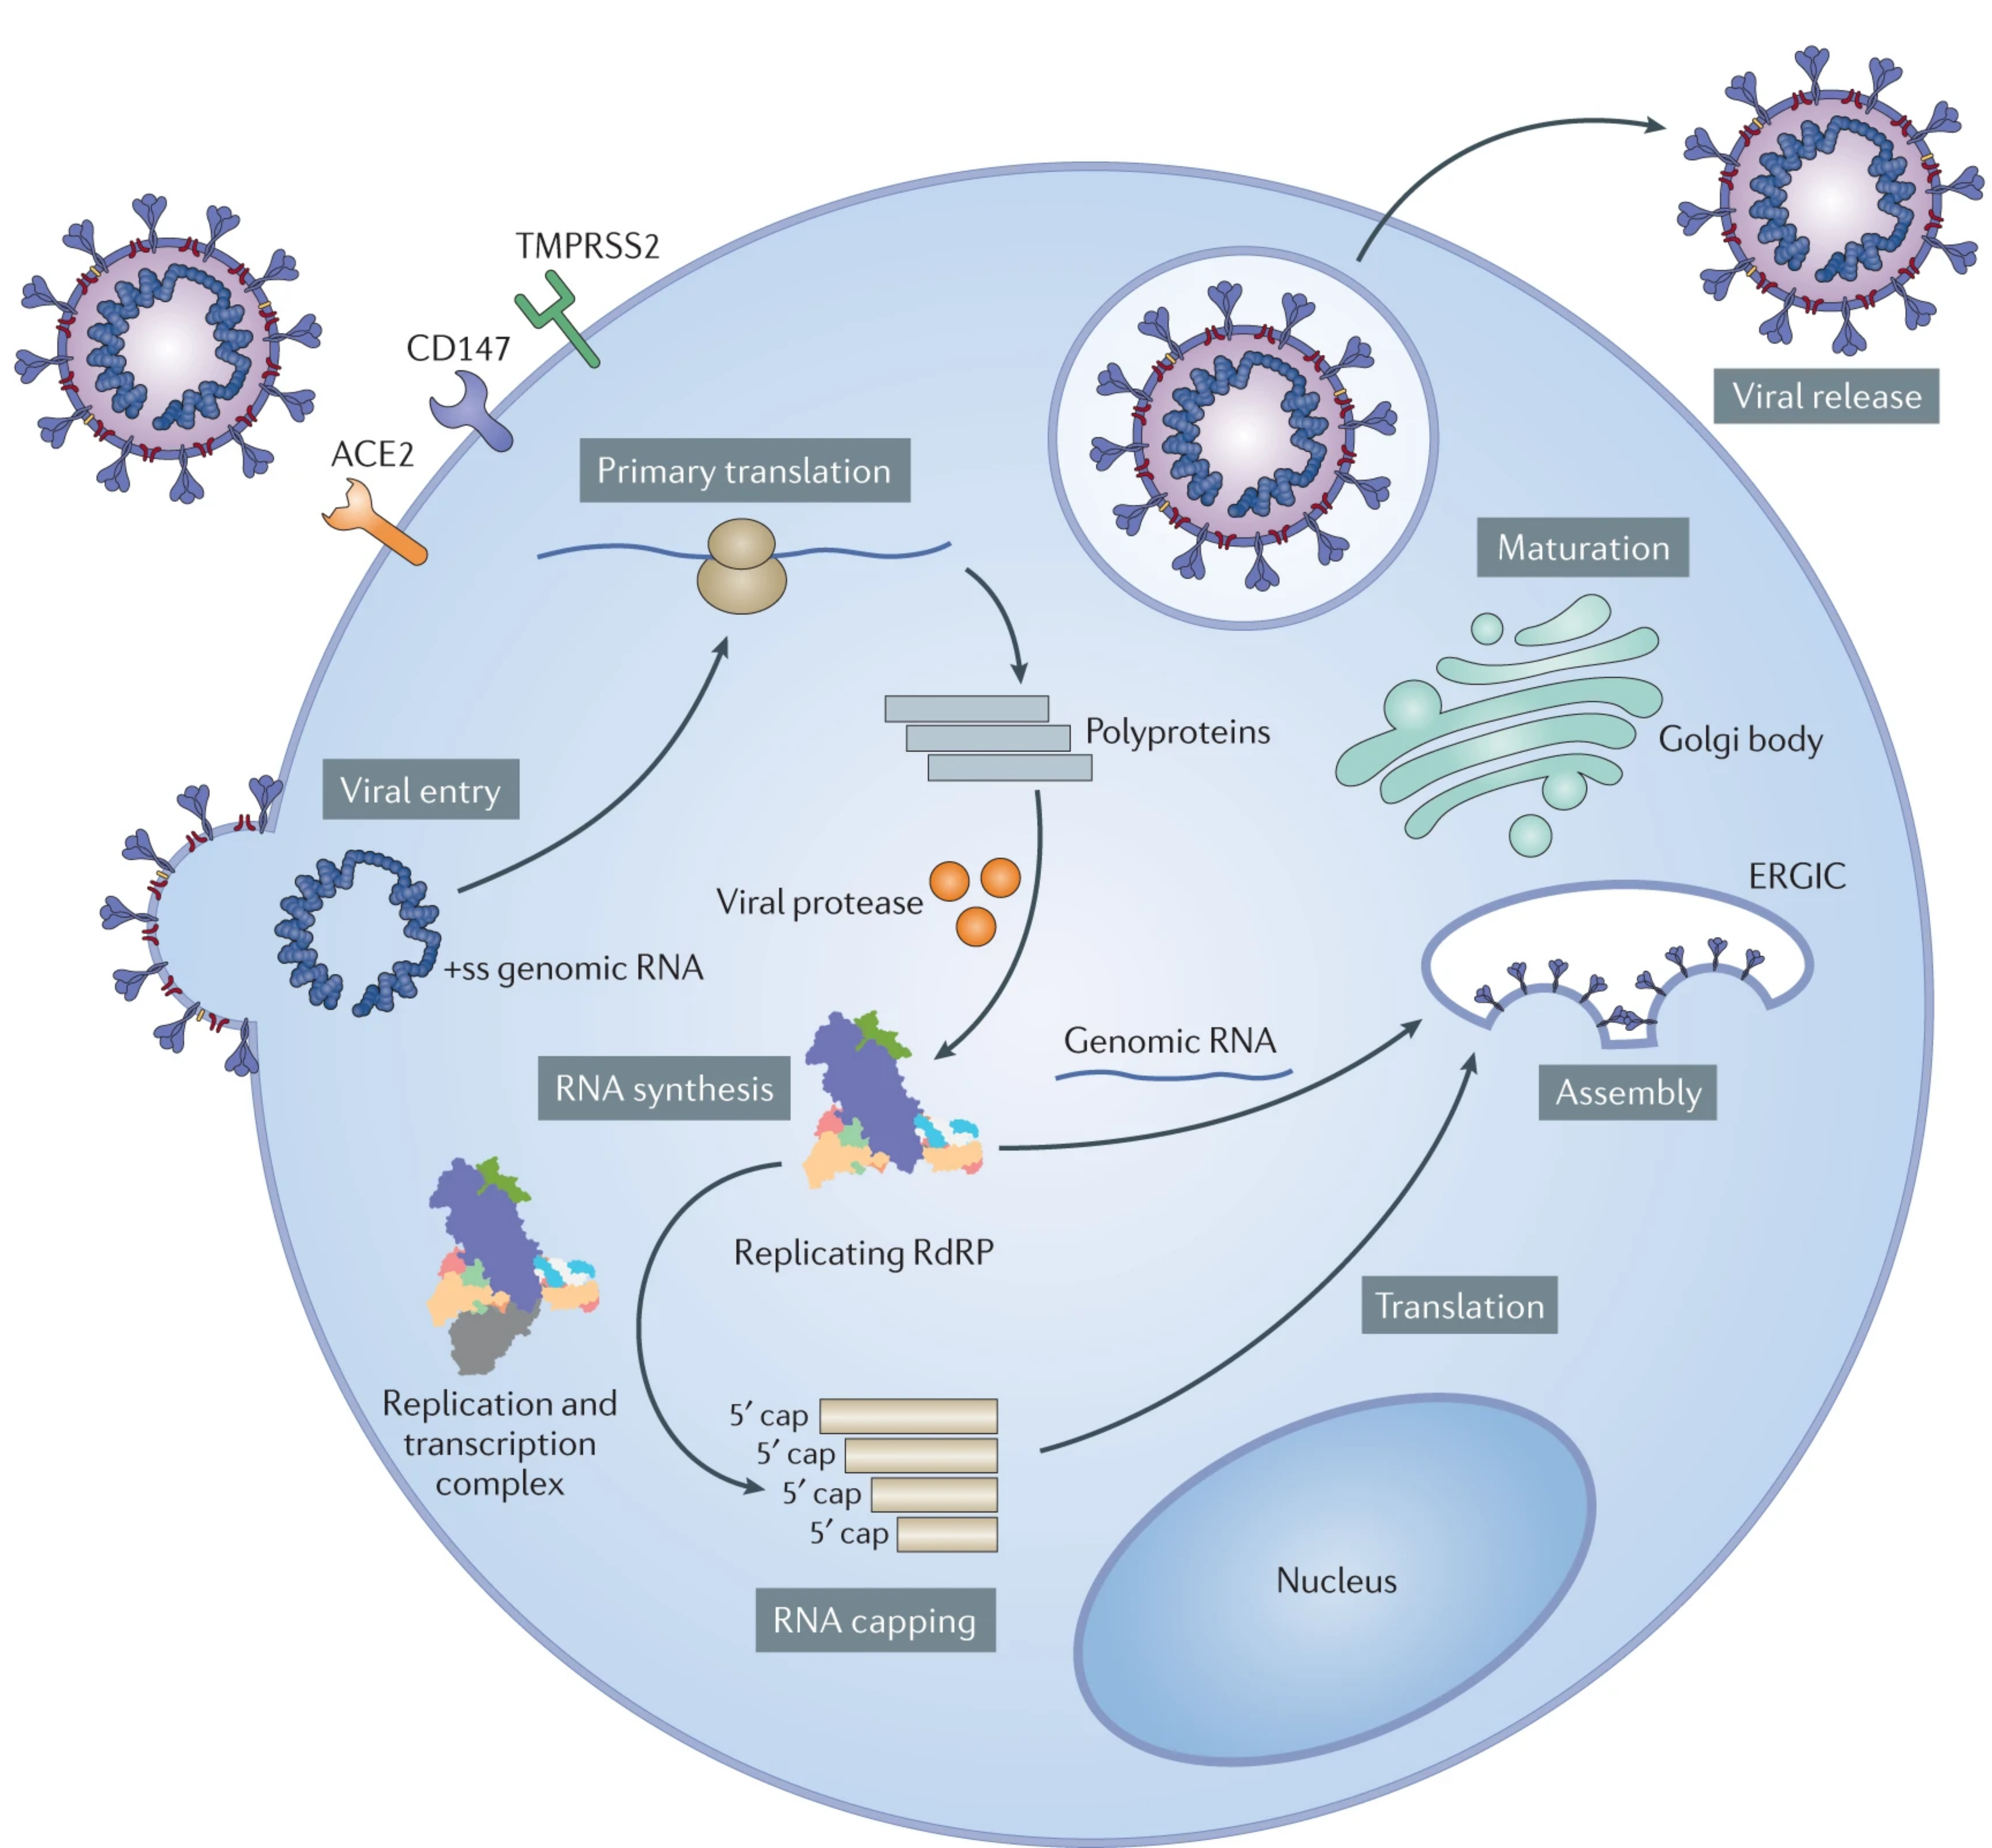
\includegraphics[width=0.7\textwidth]{Figuras/fig2.png}
    \label{fig:fig2}
    \begin{minipage}{0.7\textwidth} % Adjust width as needed
        \centering
        \footnotesize Fonte: \citeonline{Yang:2021}
    \end{minipage}

\end{wrapfigure}

\begin{wrapfigure}{c}{0pt}
\end{wrapfigure}

\vspace{10mm}

Durante o ciclo da infecção viral, algumas organelas se auto-replicam a partir do retículo endoplasmático (RE) e propiciam um ambiente favorável para replicação e transcrição de mRNAs subgenômicos (\textit{sg-mRNAs}). Aparentemente, esse mecanismo de replicação é evitado no citosol, provavelmente, para não ser detectado por sensores do sistema imune inato \cite{Vkovski:2021}. As proteínas estruturais que são traduzidas no RE acabam sendo translocadas entre as membranas do RE até o Complexo de Golgi por meio de um compartimento intermediário, onde o vírion resultante é formado.  Por fim, o vírion formado é secretado por exocitose para seguir com o ciclo de infecção nas demais células do hospedeiro \cite{Vkovski:2021, Yang:2021}.



\section{NetMHCpan: Predição de afinidade de ligação entre MHC e antígenos virais}


A identificação de epítopos de células T é um grande desafio devido à significativa variação em seu reconhecimento entre indivíduos. Os genes envolvidos com o sistema HLA são os mais diversos do genoma humano, além dos fatores ambientais que afetam o histórico de interação entre o sistema de apresentação de antígenos. As moléculas de MHC apresentam especificidades de ligação distintas, caracterizando um sistema de apresentação de epítopos robusto e variado. Na Figura \ref{fig:fig3} é possível verificar a quantidade de interações que podem ser geradas a partir da ligação entre o MHC e o peptídeo.

\begin{wrapfigure}{c}{\textwidth}
    \centering
    \caption{\justifying Resíduos âncoras Leucina e Valina de um peptídeo ALGIGILTV na fenda de HLA-A*02:01. }
    \includegraphics[width=0.7\textwidth]{Figuras/fig3.png}
    \label{fig:fig3}
    \begin{minipage}{0.7\textwidth} % Adjust width as needed
        \centering
        \footnotesize Fonte: \citeonline{Perez:2022}
    \end{minipage}
\end{wrapfigure}

\begin{wrapfigure}{c}{0pt}
\end{wrapfigure}

\vspace{10mm}

A ligação de peptídeos ao MHC é uma etapa necessária para que o sistema imune adaptativo e inato possa ser ativado, esses ligantes são classificados como epítopos de células T. Essa etapa representa o processo mais seletivo da via de reconhecimento de antígenos e compreender os mecanismos que influenciam esse evento contribui para o desenvolvimento de ferramentas, as quais  podem predizer potenciais alvos que ativam ou não uma resposta imune por meio de vias dependentes de MHC \cite{Peters:2020}. 

Essas aplicações corroboram com os avanços no desenvolvimento de vacinas, imunoterapia do câncer e pesquisa de doenças infecciosas. Por isso, múltiplos esforços são aplicados no desenvolvimento de métodos computacionais capazes de acuradamente predizer a ligação de peptídeos e mapear os epítopos ao MHC-I e MHC-II. Entre eles, existem o SYFPEITHI \cite{Rammensee:1999}, netMHCpan \cite{Reynisson:2020}, MHCflurry \cite{Odonnell:2020}, MHCnuggets \cite{Shao:2020} e MixMHCpred \cite{Gfeller:2023}.

De acordo com \citeonline{Peters:2020}, esses métodos computacionais são responsáveis por mapear os epítopos de células T que evoluíram ao longo do tempo, adicionando características a cada versão. Inicialmente, visava-se identificar os \textit{motifs} formados pelos aminoácidos dos peptídeos, os quais correspondiam aos resíduos de ligação ao MHC. Determinadas posições desses peptídeos permitem um limitado número de substituintes e com propriedades de cadeia-laterais semelhantes, os quais mantêm o potencial de ligação MHC-ligante. Esses resíduos foram chamados de resíduos âncoras e outros influentes foram classificados como auxiliares, os quais também possuíam um espaçamento e especificidade determinante para afinidade de ligação que quando somados caracterizavam os motifs dos resíduos ligantes ao MHC (Figura \ref{fig:fig4}A).

Em um segundo momento, esses métodos foram aprimorados para abordagens quantitativas da afinidade de ligação do MHC utilizando abordagens de aprendizado de máquina.  Nesse sentido, uma abordagem inicial foi determinar pontuações, a partir de valores heurísticos, para os vinte aminoácidos em cada posição que quantitativamente representasse o  seu impacto esperado. Esses valores eram estimados a partir de dados experimentais e eram derivados para se obter uma pontuação final de uma sequência peptídica em relação à determinada variante de MHC. A partir da eficiência do método heurístico, abordagens baseadas em aprendizado de máquina supervisionado foram implementadas (Figura \ref{fig:fig4}B).

Em uma terceira abordagem, as atuais ferramentas utilizam arquiteturas de redes neurais artificiais especializadas para integrar informações das interações lineares e não-lineares a partir da sequência do MHC e dados da ligação MHC-ligante. No entanto, dados experimentais são um limitante para o treinamento supervisionado, dado o número de variantes existentes. Essa limitação motivou o desenvolvimento de técnicas que baseiam-se na construção de matrizes virtuais que caracterizam o perfil de ligação de determinada variante de MHC, sem dados experimentais, por meio da comparação  dos resíduos do sulco de ligação do MHC com os resíduos do sulco de ligação de variantes que foram avaliados experimentalmente. Essa última abordagem ficou conhecida como \textit{pan-specific}, exibindo alta confiabilidade na predição de epítopos  para variantes MHC sem dados experimentais (Figura \ref{fig:fig4}C).

\begin{wrapfigure}{c}{\textwidth}
    \centering
    \caption{\justifying Representação das metodologia computacionais desenvolvidas para predição de epítopos de células T baseada em (A) \textit{motifs}, (B) métodos quantitativos heurísticos e (C) redes neurais artificiais.  }
    \includegraphics[width=0.7\textwidth]{Figuras/fig4.png}
    \label{fig:fig4}
    \begin{minipage}{0.7\textwidth} % Adjust width as needed
        \centering
        \footnotesize Fonte: \citeonline{Peters:2020}
    \end{minipage}
\end{wrapfigure}

\begin{wrapfigure}{c}{0pt}
\end{wrapfigure}

\vspace{10mm}

O primeiro método computacional a implementar predições \textit{pan-specific}  em redes neurais para moléculas do MHC Classe I foi o NetMHCpan \cite{Hoof:2009}. Esse método complementa a informação sobre a ligação MHC-ligante e ligante eluído no treinamento do modelo preditivo com informações sobre os aminoácidos que definem o sulco de ligação do MHC. Além disso, a partir de aprimoramentos, o NetMHCpan-4.1 permite desambiguar peptídeos que tiveram baixa resolução de anotação para determinados alelos a partir de dados experimentais e aumento a performance de predição em relação à demais ferramentas \cite{Reynisson:2020}.

Portanto, nesse trabalho, busca-se implementar a ferramenta NetMHCpan-4.1 na avaliação dos efeitos na ligação entre peptídeo-MHC a partir dos dados de mutações \textit{missense} de variantes de SARS-CoV-2 identificadas em Foz do Iguaçu/PR. 

\end{justify}



\chapter{Objetivos}

\begin{justify}

\section{Geral}

\hspace{12 mm}Avaliar a relação da diversidade de variantes SARS-CoV-2 que circularam em Foz do Iguaçu/PR, entre 2020 e 2022, e o impacto das mutações \textit{missense} na afinidade de ligação dos epítopos aos complexos de apresentação de antígeno HLA-B. 

\section{Específicos}

\begin{itemize}
    \item Identificar os sítios de mutações \textit{missense} mais relevantes a partir do alinhamento das variantes identificadas entre 2020 e 2022 no GISAID;

    \item Coletar os grupos alélicos de HLA-B mais frequentes no Estado do Paraná via \textit{Allele Frequency Net Database} e estudos prévios;

    \item Estimar a afinidade de ligação dos peptídeos de referência e mutados em relação aos alelos HLA-B selecionados utilizando NetMHCpan-4.1.

    \item Relacionar as mutações \textit{missense}, o período de circulação da variante e o impacto na apresentação de epítopos baseado nos dados preditos.
\end{itemize}

\end{justify}
\chapter{Materiais e Métodos}

\begin{justify}

\hspace{12 mm} Os dados experimentais foram extraídos de projetos prévios e descritos nesse trabalho. A análise das mutações \textit{missense} das variantes de SARS-CoV-2 utilizou-se de abordagens computacionais e dados públicos. As etapas computacionais de coletas das sequências genômicas, identificação das mutações e predição de epitopos  foram baseadas em metodologias prévias \cite{Hamelin:2022}.  


\section{Estudo Experimental}

O município de Foz do Iguaçu, no sul do Brasil, faz fronteira com Paraguai e Argentina. O município tem 258.823 habitantes, uma densidade de 414,58 pessoas por km², urbanização superior a 99\% e um Índice de Desenvolvimento Humano de 0,751. A rede de saúde inclui 36 unidades, sendo quatro hospitais, organizados em cinco distritos. O primeiro caso de COVID-19 foi registrado em 12 de março de 2020, seguido pelo primeiro caso de transmissão local em 25 de março, transmissão comunitária em 7 de abril e o primeiro óbito em 26 de abril.  As medidas de distanciamento social foram iniciadas a partir de 15 de março \cite{Viana:2021}.

Os pacientes COVID-19 positivo admitidos na Unidade de Tratamento Intensivo (UTI), no Hospital Municipal Paulo Germano Lauck, entre 2020 e 2021, foram submetidos à análise genotípica de HLA-B. Os indivíduos foram selecionados priorizando o histórico hospitalar e quadro clínicos melhor documentados durante o período de internação.  A pesquisa fez parte da  Ação 9 de enfrentamento a COVID-19 no âmbito da Universidade Federal da Integração Latino-Americana – Unila, intitulada “Medicina personalizada para tratamento de pacientes COVID-19 em Foz do Iguaçu” (PORTARIA No 193/2020/GR) (ProjCOVID).

\section{Aspectos Éticos}

Essa etapa faz parte do projeto "Perfil da população do oeste paranaense acometido de Síndrome Respiratória Aguda Grave entre 2020 a 2022", aprovado pelo Comitê de Ética em Pesquisa Envolvendo Seres Humanos, CAAE 36189220.3.0000.8527, em 2020,  Número do Parecer: 4.250.900.

\section{Seleção de indivíduos COVID-19 positivo}

As amostras foram coletadas de pacientes admitidos e apresentando testes RT-qPCR positivos anteriormente ou na admissão hospitalar. A coleta foi realizada a partir de julho/2020 à novembro/2020 e maio/2021 à julho/2021. Os pacientes com declaração de nacionalidade estrangeira, tempo de internação no Hospital superior à 65 dias (considerados \textit{outliers}) e que apresentam resultados ambíguos para os genótipos dos grupos alélicos de HLA foram removidos desta análise. 

O histórico hospitalar foi consultado por meio do Sistema de Gestão Tasy (Koninklijke Philips N.V, Inc., Amsterdam, NL) utilizado pelo Hospital Municipal Padre Germano Lauck, assim como, os quadros clínicos atuais foram coletados no projeto ProjCOVID. 

\section{Fase laboratorial}

De cada paciente foram coletados cerca de 6 ml de sangue periférico em tubo contendo anticoagulante EDTA (Tubo Greiner Bio-One) e armazenados em refrigeração - 80$ ͦ^\circ C$ pela equipe de enfermagem hospitalar. As amostras tiveram o DNA extraído via kit extração \textit{Geno Plus Mini} VIOGENE, numerados e armazenados no banco de amostras do LPCM-UNILA . A quantificação de cada amostra foi realizada em espectrofotômetro NanoDrop ND2000 (Thermo Fischer Inc., Waltham, MA, EUA).

Os éxons de HLA classe I \textit{loci} B foram genotipados por Sequenciamento de Grupo Específico (GSSP) via kit   \textit{SeScore Sequencing}  GSSP (One Lamda, Inc), a partir de amostras do DNA extraído dos pacientes SARS-CoV-2 positivo. As amostras foram checadas, purificadas e sequenciadas em sequenciador automático de \textit{DNA ABI 3500} (Thermo Fischer Inc., Waltham, MA, EUA). As análises dos dados obtidos foram realizadas em Software uTYPE Dx HLA \textit{Sequence Analysis} (One Lambda, Inc). Eventualmente algumas amostras apresentaram resultados com ambiguidade em baixo nível de resolução (grupos alélicos), essas amostras foram filtradas. 

\section{Estudo computacional}

Os métodos computacionais buscaram coletar os dados genômicos de variantes que circularam no município de Foz do Iguaçu (Paraná, Brasil) (Figura \ref{fig:fig5}A e \ref{fig:fig5}B), identificação de mutações missense (Figura \ref{fig:fig5}C e \ref{fig:fig5}D), predição da afinidade de ligação de peptídeos virais mutados (Figura \ref{fig:fig5}E e \ref{fig:fig5}F) e análise descritiva e estatística (Figura \ref{fig:fig5}G). Além disso, dados experimentais de projetos anteriores foram utilizados para direcionar a escolha dos alelos HLA-B selecionados neste estudo.

\begin{wrapfigure}{c}{\textwidth}
    \centering
    \caption{\justifying Etapas do \textit{pipeline} para análise das mutações \textit{missense}. Coletas de dados genômicos (A), alinhamento das sequências das mesmas variantes (B), alinhamento das sequências consenso de cada variante com a sequência de referência (C), identificação de mutações \textit{missense} (D), geração dos peptídeos de referência e mutados (E), predição da afinidade de ligação (F) e análise estatística (G). Quadros vermelhos apresentam dados quantitativos de cada etapa. }
    \includegraphics[width=1\textwidth]{Figuras/fig5.png}
    \label{fig:fig5}
    \begin{minipage}{0.8\textwidth} % Adjust width as needed
        \centering
        \footnotesize Fonte: O Autor (2024)
    \end{minipage}
\end{wrapfigure}

\begin{wrapfigure}{c}{0pt}
\end{wrapfigure}

\section{Coleta de dados genômicos}

As 655 sequências genômicas de SARS-CoV-2 foram coletadas via GISAIDR (versão 0.9.10) \cite{Wirth:2022} a partir do banco de dados EpiCoV, pertencente ao \textit{Global Initiative on Sharing All Influenza Data} (GISAID) \cite{Khare:2021}. A requisição foi realizada para sequências genômicas completas ($\geq$29kb) coletadas entre 01/01/2020 e 01/01/2023, extraídas a partir de amostras provenientes da cidade de Foz do Iguaçu - Paraná/Brasil (Figura \ref{fig:fig5}A e \ref{fig:fig5}B). As 55 variantes detectadas foram inferidas com base na classificação fornecida pelo \textit{EpiCoV}. Sequências com mais de 5\% das bases desconhecidas, extraídas de amostras ambientais ou variantes que tiveram apenas uma sequência coletada foram excluídas. O banco de sequências utilizado neste estudo pode ser acessado via
 \href{http://gisaid.org/EPI_SET_240517bd}{gisaid.org/EPI\_SET\_240517bd}.

\section{Identificação de mutações \textit{missense} de SARS-CoV-2}

As sequências consenso foram obtidas a partir de sequências alinhadas de mesma variante. A sequência de referência SARS-CoV-2 Wuhan-1 (NC\_045512.2) foi alinhada com cada sequência consenso individualmente utilizando \textit{minimap2 v2.26-r1175}. As sequências mapeadas foram  ordenadas e convertidas em um arquivo \textit{.bam} utilizando \textit{samtools v1.18}. A chamada das variantes foi realizada utilizando \textit{bcftools mpileup v1.17} no modo haplóide e mutações somáticas foram anotadas a partir de \textit{snpEff v4.3} com a função \textit{ann} (Figura \ref{fig:fig5}D).

\section{Predição da afinidade de ligação de peptídeos virais mutados}

Os peptídeos virais foram selecionados a partir da posição de mutação, gerando \textit{k-mers} de 10 à 14 aminoácidos com a presença de mutação única em cada uma das posições, assim como, peptídeos não mutados como referência (Figura \ref{fig:fig5}E). Os peptídeos que apresentavam similaridade e identidade completa com peptídeos do genoma humano \textit{GRCh38} foram descartados utilizando o \textit{Ensembl BioMart} \cite{Harrison:2024, Kinsella:2011}. A afinidade de ligação dos peptídeos virais selecionados foi predita contra 15 alelos de HLA-B (B*07:02, B*08:01, B*14:02, B*15:01, B*18:01, B*27:05, B*35:01, B*38:01, B*39:01, B*40:01, B*44:03,  B*49:01,  B*51:01, B*53:01, B*57:01). A escolha dos alelos teve como base os grupos alélicos presentes nas coletas experimentais realizadas em 2020  e 2021 pelo laboratório, além de acrescentar alelos frequentes no Estado Paraná detectados no Registro Brasileiro de Doadores Voluntários de Medula Óssea (REDOME) e em estudos prévios (Apêndice A).

A predição da afinidade de ligação dos peptídeos foi realizada pelo NetMHCpan 4.1 EL, esse método utiliza uma rede neural treinada com dados experimentais de afinidade de ligação e dados de ligantes eluídos para gerar uma pontuação que indica a probabilidade de um peptídeo ser um ligante para os tipos de HLA especificados \cite{Reynisson:2020}. A probabilidade de ligação é expressa em forma de classificação percentílica (\%rank), onde os ligantes classificados como fracos (\textit{Weak binder}, WB) obtiveram um \%rank abaixo de 2.0, enquanto os ligantes fortes (\textit{Strong binder}, SB) obtiveram um \%rank abaixo de 0.5 ou não ligantes (\textit{Non binder}, NB) obtêm um \%rank acima de 2.0 (Figura \ref{fig:fig5}E). 

Com base nesse sistema de classificação, os pares de peptídeos referência/mutados que apresentaram uma transição de classificação a partir das mutações foram reclassificados com base na perda ou ganho de afinidade de ligação. As mutações que fizeram peptídeos passar de ligantes fortes (SB) para ligantes fracos (WB) ou não-ligantes (NB) levam a classificação de uma leve perda (Weak loss) ou uma perda de ligação (Loss), respectivamente. Enquanto que mutações que causam um ganho de afinidade de ligação de WB para SB ou de NB para SB foram consideradas como um leve ganho de ligação \textit{Weak gain} ou \textit{Gain}, respectivamente (Figura \ref{fig:fig5}F e \ref{fig:fig6}).

\begin{wrapfigure}{c}{\textwidth}
    \centering
    \caption{\justifying Esquema demonstrando o conceito de perda (\textit{Loss}) e ganho (\textit{Gain}) de afinidade de ligação dos epítopos de referência e mutados. }
    \includegraphics[width=0.7\textwidth]{Figuras/fig6.jpg}
    \label{fig:fig6}
    \begin{minipage}{0.8\textwidth} % Adjust width as needed
        \centering
        \footnotesize Fonte: \citeonline{Hamelin:2022}
    \end{minipage}
\end{wrapfigure}

\begin{wrapfigure}{c}{0pt}
\end{wrapfigure}

\section{Análise estatística}

O teste não-paramétrico de Sinais de Wilcoxon foi aplicado para definir a significância estatística entre os valores de \%rank para peptídeos de referência e mutantes em relação a cada alelo analisado (Figura \ref{fig:fig5}F). A amplitude de impacto de cada mutação que gerou perda na afinidade de ligação foi analisada por meio da equação \eqref{eq:fc}, transformação \textit{log} a partir do valor de \%rank com mutação normalizado em relação ao \%rank de referência:
%

\begin{subequations}
\begin{gather}

\log_2(Fold\;Change) = \log_2(\dfrac{\%rank_{mutação}}{\%rank_{referência}})   \label{eq:fc} 

\end{gather}
\end{subequations}


Os grupos alélicos detectados no Estudo Experimental foram organizados pela data de admissão hospitalar e grupos alélicos que foram detectados em menos de 10 pacientes, entre 2020 e 2021, foram agrupados em "Outros". Os p-valores das comparações das frequências de HLA-B entre os grupos foram obtidos por Teste Exato de Fisher ao nível de significância adotado de 5\% (\( p < 0.5 \)). Quando mencionado, os p-valores foram ajustados para múltiplas comparações com o método de Bonferroni. 

\section{Modelo Estrutural}

O modelo estrutural da glicoproteína spike (na forma clivada no sítio de clivagem da furina) com uma ligação ao ACE2 foi utilizado a partir dos conjuntos de coordenadas do PDB ID:7A94 \cite{Benton:2020}. O software Pymol (The PyMOL Molecular Graphics System, v.2.2.0) foi empregado para visualização.

\section{Ferramentas Computacionais}

O \textit{pipeline} foi construído com Nextflow v23.10.1.5891 e as diferentes etapas para predição da afinidade de ligação foram executadas via Python 3.10, utilizando um script adaptado a partir do \textit{pipeline nf-core/epitopeprediction v2.2.1} \cite{Mohr:2024}.  As análises de dados e gráficos foram produzidos no software RStudio v2023.06.02 (R versão 4.4). Os códigos e os dados estão disponíveis em \href{https://github.com/chagas98/sarscovHLAFoz}{github.com/chagas98/sarscovHLAFoz}.

\end{justify}
\chapter{Resultados e discussão}

\begin{justifying}
\section{Diversidade genômica de SARS-CoV-2 em Foz do Iguaçu - Paraná/BR}

No total, excluindo sequências de amostras ambientais, 640 sequências foram utilizadas nas análises. De acordo com a classificação realizada pelo GISAID, foram detectadas 34 variantes em Foz do Iguaçu/PR no período entre 01/01/2020 e 01/01/2023. A quantidade de genomas sequenciados foram 9 (1.5\%), 265 (45.68\%), 197 (33.96\%) e 109 (18.7\%) para a primeira onda (Fev/2020 a Out/2020) , segunda onda (Nov/2020 a Dez/2021), terceira onda (Jan/2022 a Mai/2022) e o segundo semestre de 2022, respectivamente (Figura \ref{fig:fig7}A). 

Essa diversidade genômica contribui para compreender a prevalência das mutações durante as ondas epidemiológicas de SARS-CoV-2. Na cidade da tríplice fronteira, a primeira onda foi marcada pela presença das variantes B.1.1.28 e B.1.1.33. A segunda onda foi marcada pela predominância das variantes P.2 (Zeta), P.1 (Gamma), P.1.7 (Gamma) e sub-linhagens Delta (AY.101, AY.99.2, AY.46.3 e AY.122), respectivamente. A terceira onda  (Jan/2022 a Mai/2022) possuiu uma maior diversidade de variantes em relação às duas primeiras fases, sendo marcada majoritariamente pela circulação de sub-linhagens Ômicron/BA.1.* e BA.2.*. No segundo semestre de 2022, houve uma predominância da variante Ômicron/BA.5.2.1 em relação às demais variantes, assim como, uma diminuição no número de genomas sequenciados.

As variantes Gamma e Zeta surgiram durante a segunda onda, com a variante Gamma emergindo ao final do mês de Novembro/2020, no município de Manaus/AM. Enquanto a variante Zeta foi descrita em Outubro/2020, no município do Rio de Janeiro/RJ. No entanto, estudos anteriores apresentam indícios do surgimento da variante Zeta no estado do Paraná ao final de Agosto/2020, tendo detecções originadas em diferentes localidades da região Sul e Sudeste \cite{Faria:2021, Giovanetti:2022}. Essa constatação é similar com o comportamento epidemiológico observado no município de Foz do Iguaçu, onde a Zeta foi detectada dois meses antes da Gamma (Figura \ref{fig:fig7}A).

Ao final da segunda onda, as variantes Delta foram detectadas majoritariamente. Com exceção da Venezuela e Guianas, países da América do Sul não tiveram uma ressurgência com essas variantes \cite{Graf:2024}. No entanto, sua prevalência no sul brasileiro foi notória em relação às demais linhagens, tendo indícios do surgimento da AY.101 no Estado do Paraná \cite{Arantes:2022}.

\begin{wrapfigure}{c}{\textwidth}
    \centering
    \caption{\justifying Diversidade de linhagens de SARS-CoV-2 em Foz do Iguaçu/PR de Mar/2020 a Dez/2022. (A) Prevalência relativa das linhagens ao longo dos meses, quadro superior apresentando o número de genomas sequenciados, linhas superiores demonstrando o período das ondas de acordo com estudos prévios \cite{Bastos:2021, Giovanetti:2022, Graf:2024, Moura:2022}; (B) perfil alélico de pacientes do HMPGL obtido a partir do estudo experimental, quadro superior apresentando o número de amostras sequenciadas. Mês correspondente a data de detecção/admissão.}
    \includegraphics[width=1\textwidth]{Figuras/fig7.png}
    \label{fig:fig7}
    \begin{minipage}{0.8\textwidth} % Adjust width as needed
        \centering
        \footnotesize Fonte: O Autor (2024)
    \end{minipage}
\end{wrapfigure}

\begin{wrapfigure}{c}{0pt}
\end{wrapfigure}

\vspace{10mm}

A composição das variantes das duas primeiras ondas foi comparada de forma indireta com o perfil alélico de pacientes admitidos no HMPGL. O estudo experimental obteve o resultado de 74 amostras de pacientes COVID-19, sendo 27 coletados em 2020 e 47 coletados em 2021. O perfil alélico foi obtido para os genes de HLA-B em uma resolução baixa a nível de grupos alélicos, amostras ou resultados com ambiguidades não foram tratados. Alelos que apresentaram um número total de ocorrências inferior a dez foram agrupados em ``Outros'' (Figura \ref{fig:fig7}B).

O B*07 apresentou diferença significativa entre os anos de coleta (p = 0.02) e óbitos (p = 0.004) em 2020 e 2021, esse último sugerindo uma mudança na ocorrência em pacientes com alta e óbito (Tabela \ref{tab1}). Já o B*41 apresentou diferença entre os desfechos para 2020, mas não atingiu o limiar de significância. Quando ajustado os p-valores para múltiplas comparações, no entanto, os p-valores perdem significância. O grupo alélico B*35 apresentou diferença entre os desfechos de cada ano, mas não foi detectada significância. 

\begin{table}[!h]{14cm}
\caption{Comparações entre as Frequências dos Grupos Alélicos.}\label{tab1}
\scalebox{0.8}{
	\begin{tabular}{ccccccccc}
            \rowcolor[HTML]{999999} 
		\hline
		\textbf{Alelos} 
            & \textbf{\textit{p}} 
            & \textbf{\textit{p.adj}} 
            & \textbf{G1$^1$} 
            & \textbf{G2$^2$}
            & \textbf{G1(n)} 
            & \textbf{G2(n)} 
            & \textbf{Outros 1 (n)} 
            & \textbf{Outros 2 (n)} \\ 
		\hline
		B*41 & 0.052 & 1.0 & Alta20 & Óbito20 & 5 & 0 & 23 & 26 \\
            \rowcolor[HTML]{CCCCCC} 
		B*07 & 0.020 & 0.47 & 2021 & 2020 & 5 & 10 & 89 & 44 \\
            \rowcolor[HTML]{FFFFFF} 
		B*07 & 0.004 & 0.1 & Óbito20 & Óbito21 & 7 & 1 & 19 & 41 \\
		\hline
	\end{tabular}}
        \begin{tablenotes}\footnotesize
         \raggedright
            \item \scriptsize\textit{$^1$}Grupo 1 
            \item \scriptsize\textit{$^2$}Grupo 2
            \par
        \end{tablenotes}
	%\legend{Texto da legenda. (opcional)}
	\source{O Autor (2024)}
\end{table}

Além disso, quando comparadas as frequências relativas com as frequências coletadas do REDOME, o grupo alélico B*07 apresentou uma diferença percentual evidente entre 2020 (18\%), 2021 (5\%) e REDOME (7\%).

\section{Diversidade de mutações \textit{missense} concentra-se em \textit{ORF1ab} e \textit{spike}}

A partir das sequências genômicas, foram gerados 8.222 peptídeos entre \textit{10mers} e \textit{14mers} proveniente das posições de 185 mutações únicas identificadas. As regiões com maior número de mutações \textit{missenses} foi a \textit{ORF1ab} (58), \textit{spike - S} (56) e \textit{Nucleocapsídeo - N} (20), as regiões restantes tiveram menos de 10 mutações. No entanto, a glicoproteína \textit{spike} e as poliproteínas \textit{ORF1ab}  apresentaram maior número de mutações classificadas em \textit{Loss}, 4 e 3, respectivamente. Enquanto a proteína \textit{N} apresentou uma única mutação com forte perda (\textit{Loss}) de afinidade de ligação (Figura \ref{fig:fig8}A).

Além disso, a afinidade de ligação foi mensurada para cada agrupamento. No entanto, como os epítopos não mutados são previstos como não ligantes, essas mutações não foram comparadas com a lista de epítopos validados com alta afinidade de ligação. Ainda é necessário determinar experimentalmente se as mutações do SARS-CoV-2 que aumentam a afinidade dos epítopos ao HLA podem melhorar as respostas das células T e auxiliar no controle do vírus em pacientes com COVID-19.

\begin{wrapfigure}{c}{\textwidth}
    \centering
    \caption{\justifying Número de mutações únicas que levaram ao efeito de (\textit{Weak}) \textit{Gain} ou (\textit{Weak}) \textit{Loss} para (A) cada \textit{ORF}, (B) cada variante e (C) cada alelo. A contagem considera os efeitos para cada alelo predito. Figura B possui as variantes por ordem da primeira detecção na cidade de Foz de Iguaçu de baixo para cima.
}
    \includegraphics[width=1\textwidth, height=0.5\textwidth]{Figuras/fig8.png}
    \label{fig:fig8}
    \begin{minipage}{0.8\textwidth} % Adjust width as needed
        \centering
        \footnotesize Fonte: O Autor (2024)
    \end{minipage}
\end{wrapfigure}

\begin{wrapfigure}{c}{0pt}
\end{wrapfigure}

\vspace{10mm}

Por outro lado, algumas regiões não possuíram mutações com impacto negativo na predição de afinidade por epítopos. Por exemplo, o envelope apresentou uma única mutação e que não causou qualquer impacto negativo nas análises de afinidade de ligação,  a mutação T9I (posição 9, T$\,\to\,$I) prevaleceu ao longo de 23 variantes. Estudos anteriores sugerem que essa mutação pode estar relacionada à ineficiência do canal de íons transmembrana do vírus, reduzindo a cascata de sinalização intracelular,  resultando em uma diminuição da produção citocinas e diminuição da virulência. Esses fatores podem ter contribuído pelo seu surgimento em Março/2020 e prevalência ao longo das variantes Alfa, Beta, Gamma e Delta em 0,20\%, chegando a 100\% de ocorrência nas variantes Ômicron \cite{Xia:2022}.

Em Foz do Iguaçu, a mutação T9I possivelmente foi introduzida através das variantes Ômicron (BA.*) e tiveram prevalência em variantes posteriores, de BA.1.1 até BE.10. Essa tendência de prevalência pode ser observada na chegada de outras variantes além da Ômicron, as quais contribuíram para o aumento de epítopos mutados que tiveram perda de afinidade de ligação preditas, como no caso das variantes Gamma (P.1 + P.1.7), Zeta (P.2), Delta (AY.101 + AY.99.2 + AY.46.3) (Figura 8B).

Em \textit{ORF1ab}, as mutações com maior prevalência são P323L/P4715L (34), as quais são provenientes da mutação 14408C\textgreater U à nível de nucleotídeo. Esta mutação resulta em uma mutação \textit{missense} P4715L a nível de aminoácidos da poliproteína \textit{ORF1ab} e aparece como mutação P323L na enzima RNA-polimerase RNA-dependente (RdRp). Essa mutação teve uma perda suave na afinidade de ligação em relação ao alelos B*15:01, em conformidade com os relatos da associação dessa mutação com casos severos e elevação na taxa de mortalidade \cite{Toyoshima:2020}.

Outras mutações com frequência significativa em \textit{ORF1ab}, como S135R (13) e P132H/P3395H (23) foram classificados como \textit{Loss}, com as duas últimas mutações levando uma perda de epítopos B*07:02. Esse fato corrobora com análises de bioinformática prévias, as quais sinalizam a perda  de afinidade de epítopos em relação aos alelos HLA-B7 \textit{supertype} \cite{Hamelin:2022}. Na Figura 8C, é possível observar uma tendência dos alelos B*07:02 e B*27:02, principais representantes de HLA-B7 e HLA-B27, na perda de afinidade de ligação a partir de epítopos mutados, contendo o maior número de mutações classificadas como \textit{Loss}, respectivamente.

Em relação à glicoproteína \textit{spike}, a mutação D614G apresentou maior frequência em relação a todas as mutações detectadas na cidade de Foz do Iguaçu, ao total foram 34 variantes portadoras desta mutação (Figura \ref{fig:fig9}A). A D614G não afetou a afinidade de ligação a partir das predições realizadas para os alelos de HLA-B, apesar da sua ocorrência estar ligada ao aumento da taxa de mortalidade, aumento do sinal de detecção de RT-qPCR devido a carga viral e predições relacionadas aos alelos HLA-A \cite{Hamelin:2022, Korber:2020, Toyoshima:2020}. Por outro lado, epítopos com mutações P681H (24), P681R (4), R346K (3) e R346T (2) apresentaram uma perda significativa na afinidade de ligação aos alelos  B*27:05 e B*07:02 para as posições 681 e 346, respectivamente. Enquanto as mutações T95I (10) e V213G (14) foram classificadas como \textit{Weak Loss} em relação à  B*57:01 e B*38:01, respectivamente.  


\begin{wrapfigure}{c}{\textwidth}
    \centering
    \caption{\justifying Distribuição da posição dos epítopos e suas variantes mutadas dos antígenos de SARS-CoV-2 que circularam em Foz do Iguaçu/PR. (A) Posição das mutações ao longo do genoma de SARS-CoV-2, mutações que ocorreram em mais de 20 variantes estão destacadas em amarelo, mutações que foram classificadas como \textit{Gain}, \textit{Loss} e \textit{Weak Loss} estão destacadas em cinza escuro, vermelho e salmão, respectivamente; (B) estrutura de um monômero da \textit{spike} ligado à ACE2. As posições das mutações e região do FCS (680-690) estão destacadas em esferas vermelha e verde, respectivamente. 
}
    \includegraphics[width=1\textwidth, height=0.8\textwidth]{Figuras/fig9.png}
    \label{fig:fig9}
    \begin{minipage}{0.8\textwidth} % Adjust width as needed
        \centering
        \footnotesize Fonte: O Autor (2024)
    \end{minipage}
\end{wrapfigure}

\begin{wrapfigure}{c}{0pt}
\end{wrapfigure}

\vspace{10mm}


A mutação P681R é exclusivamente carregada por variantes Delta, já a mutação P681H surge a partir de variantes Ômicron em conjunto com mutação N679K (Figura \ref{fig:fig9}C). Essas mutações ocorrem em uma posição adjacente ao ao Sítio de Clivagem da Furina (\textit{FCS}, sigla em inglês) e aumentam o número de aminoácidos básicos, característica crucial para o reconhecimento pela furina \cite{Harvey:2021}.  Além da perda da prolina que afetam a apresentação de epítopos associados à HLA-B7 supertype, mutações na posição 681 também apresentaram resistência à beta interferon (IFN-$\beta$) e conferindo uma evasão em relação ao sistema imune adaptativo e inato \cite{Hamelin:2022, Lista:2022}. 

As mutações na posição R346 surgiram de forma tardia, R346K e R346T foram prevalentes em variantes BA.1.* e BA.4.6/BQ.1.1, respectivamente. Resultados experimentais sugerem que essas mutações podem conferir uma resistência à neutralização por anticorpos previamente identificados por atuarem em antígenos de SARS-CoV-2  \cite{Cao:2022}. A mutação V213G surge de maneira tardia a partir de BA.2.* e  a mutação T95I a partir da variante Delta AY.101 e prevalece ao longo das sub-linhagens Ômicron BA.1.*. 

A glicoproteína spike é essencial para a interação com a enzima de conversão de angiotensina 2 (\textit{ACE2}, sigla em inglês), expresso nas células hospedeiras, e é importante para a transmissão viral, sendo uma região crítica para prevalência de mutações \textit{missense} \cite{Harvey:2021, Piccoli:2020, Toyoshima:2020}. Na Figura \ref{fig:fig9}B e \ref{fig:fig9}C, é possível observar que o domínio de ligação de receptor (\textit{Receptor Binding Domain - RBD}) acumula o maior número de mutações em relação ao C-terminal e N-terminal, região de maior contato com receptores \textit{ACE2}. 

De acordo com \citeonline{Piccoli:2020},  o RBD de SARS-CoV-2 é imunodominante em relação a quantidade total de anticorpos monoclonais elicitados, é alvo de 90\% da atividade neutralizante presente no soro ou plasma de indivíduos infectados e apresenta dois sítios principais na neutralização da fusão do vírus à células hospedeiras pela ligação ao \textit{ACE2}. Além da região \textit{RBD}, as variantes Ômicron possuíram mutações conservadas (H655Y, N679K e P681H) adjacente ao \textit{FCS}, as quais potencializaram a clivagem da proteína \textit{spike} e a fusão com a célula hospedeira \cite{Viana:2022}.  

No entanto, ao contrário das variantes Alpha (P681H) e Delta (P681R), as mutações em \textit{RBD} e \textit{FCS} não foram determinantes para prevalência e alta transmissibilidade das variantes Ômicron. As mudanças genotípicas nas novas variantes do vírus demonstraram alterar o fenótipo viral, modulando as respostas imunes inatas e a evasão da resposta imune adaptativa, além de modificar a funcionalidade da proteína \textit{spike}, afetando a transmissão e a patogênese.  \cite{Harvey:2021, Willett:2022}. Segundo resultados apresentados por \citeonline{Willett:2022}, variantes Ômicron BA.1 e BA.2 mudaram a preferência de via de entrada à célula hospedeira, utilizando um mecanismo de fusão endossômica independente de TMPRSS2, principal protease transmembrana envolvida na fusão do envelope viral. 

Em Foz do Iguaçu, além da D614G, P681* e H655Y que prevalecem na \textit{spike} de diferentes variantes, as mutações mais abundantes ocorreram ao longo da circulação de sub-linhagens Ômicron, evidenciando a diversidade de mutações dessas linhagens que geraram uma série de mecanismos fenotípicos adaptados para sua prevalência ao longo do tempo.  Apesar da mutação D614G surgir amplamente nas variantes da primeira onda, a segunda mutação mais frequente H655Y é compartilhada exclusivamente entre as variantes Gamma P.1 e Ômicron BA.1.1 \cite{Ou:2022}.

\section{Epítopos de B*07:02 apresentam  maior perda na afinidade de ligação com mutações \textit{missense}}

A partir do \textit{pipeline} desenvolvido, foram detectadas 23 epítopos mutados que apresentaram impacto negativo nos valores de afinidade de ligação preditos em relação aos alelos escolhidos de HLA-B. De acordo com a Figura 10A, as variantes apresentaram um acúmulo de mutações classificadas em Weak Loss/Loss ao longo do tempo.  O surgimento de mutações com perdas leves preditas teve maior concentração em ORF1ab (Figura \ref{fig:fig10}A e \ref{fig:fig10}B) e quando ocorreram efeitos negativos, mutações na proteína \textit{spike} geraram um alto impacto na afinidade de ligação predita.

\begin{wrapfigure}{c}{\textwidth}
    \centering
    \caption{\justifying Valores de \textit{Log}$_{2}$(\textit{Fold Change}) para cada mutação classificada em (\textit{Weak}) \textit{Loss}. Mutações classificadas por (A) variantes e (B) por genes. Variantes estão ordenadas de baixo para cima a partir da primeira data de detecção em Foz do Iguaçu. Mutações que geraram Loss estão identificadas com alelo:mutação:\textit{k-mer}  e indicação na lateral esquerda da onda epidemiológica que ocorreu a primeira detecção em (B)}
    \includegraphics[width=1\textwidth, height=0.8\textwidth]{Figuras/fig10.png}
    \label{fig:fig10}
    \begin{minipage}{0.8\textwidth} % Adjust width as needed
        \centering
        \footnotesize Fonte: O Autor (2024)
    \end{minipage}
\end{wrapfigure}

\begin{wrapfigure}{c}{0pt}
\end{wrapfigure}

\vspace{10mm}

Em relação ao perfil de mutações  \textit{Weak Loss}/\textit{Loss} de cada variante, é possível visualizar que foi diferente em cada período marcado pelas ondas epidemiológicas. Como apresentado na Figura \ref{fig:fig9}A, variantes Gamma, Zeta e Delta marcam essa mudança, seguida pelas variantes Ômicron. Curiosamente, as mutações nas primeiras variantes detectadas e com menor magnitude de \textit{fold change} concentram-se em grande parte na \textit{ORF1ab}. Essa região codifica proteínas não estruturais envolvidas na replicação viral e podem tolerar mais mutações, pois estão envolvidas em processos que podem ser menos impactados por mutações pontuais.

Os epítopos mutados classificados com perda apresentaram  1.1-\textit{fold} à 120-\textit{fold} de diminuição nos valores preditos em relação à sequências de referência.  Enquanto isso, os epítopos que apresentaram maior amplitude (\textit{Log2(Fold Change)} $\geq$ 5), entre 34-\textit{fold} à 120-\textit{fold}), possuem prevalência a partir das variantes Gamma (P.1.7) e permanecem ao longo das variantes Ômicron.  As perdas são detectadas quando comparadas a epítopos de referência B*07:02, seguido dos epítopos de B*27:05 (Figura \ref{fig:fig10}B). O momento de surgimento das mutações que atingem epítopos B*07:02 difere ao período de maior número de pacientes internados que carregam o grupo alélico B*07 ao final da primeira onda, segundo os dados experimentais.

A mutação Prolina (P)$\,\to\,$X e Arginina (R)$\,\to\,$X afetam, majoritariamente, os valores preditos para  epítopos B*07:02 e B*27:05, respectivamente. Especialmente, quando localizado na posição âncora do epítopo, nesse caso, P2.  Conforme visualizado na (Tabela \ref{tab2}),   esse tipo de mutação está diretamente relacionada com o aumento da magnitude de \textit{fold change}. Dados similares foram apresentados em estudos anteriores, onde coletaram dados genômicos globais de SARS-CoV-2 e verificaram o impacto negativo nesse tipo de mutação na apresentação alélica de epítopos associados ao HLA-B7 \textit{supertype}, mas um impacto positivo foi apontado para HLA-B27 \textit{supertype}  \cite{Hamelin:2022}. 

% Please add the following required packages to your document preamble:
% \usepackage[table,xcdraw]{xcolor}
% Beamer presentation requires \usepackage{colortbl} instead of \usepackage[table,xcdraw]{xcolor}
\begin{table}[!h]{15.5cm}
\caption{Mutações \textit{Loss} epítopos associados ao alelo B*07:02 e B*27:05}\label{tab2}
\scalebox{0.7}{
\begin{tabular}{cccccccc}
\hline
\rowcolor[HTML]{999999} 
\textbf{Epítopo (Ref/mut)} &
  \textbf{K-mers} &
  \textbf{Gene} &
  \textbf{Alelo} &
  \textbf{Mutação} &
  \textit{\textbf{Log$_2$(FC)}} &
  \textit{\textbf{FC$^1$}} &
  \textbf{Núm. de variantes} \\
  \hline
R\textbf{P/H}NFTIKGSFL   & 11 & ORF1ab & B*07:02 & P132H/P3395H & 6.9  & 120.03 & 23 \\
\rowcolor[HTML]{CCCCCC} 
R\textbf{P/H}NFTIKGSF    & 10 & ORF1ab & B*07:02 & P132H/P3395H & 6.7  & 104.34 & 23 \\
S\textbf{P/R}RRARSVASQSI & 13 & S      & B*07:02 & P681R        & 5.79 & 55.57  & 4  \\
\rowcolor[HTML]{CCCCCC} 
AT\textbf{R/T}FASVYAW    & 10 & S      & B*27:05 & R346T        & 5.75 & 53.98  & 2  \\
T\textbf{R/T}FASVYAWNR   & 11 & S      & B*27:05 & R346T        & 5.43 & 43.23  & 2  \\
\rowcolor[HTML]{CCCCCC} 
S\textbf{P/H}RRARSVASQSI & 13 & S      & B*07:02 & P681H        & 5.41 & 42.72  & 24 \\
AT\textbf{R/K}FASVYAW    & 10 & S      & B*27:05 & R346K        & 3.79 & 13.85  & 3  \\
\rowcolor[HTML]{CCCCCC} 
T\textbf{R/K}FASVYAWNR   & 11 & S      & B*27:05 & R346K        & 3.62 & 12.36  & 3  \\
IPARARV\textbf{E/D}CF    & 10 & ORF1ab & B*07:02 & E341D        & 1.37 & 2.58   & 2  \\
\rowcolor[HTML]{CCCCCC} 
GPQNQRNA\textbf{P/L}RITF & 13 & N      & B*07:02 & P13L         & 1.34 & 2.54   & 24 \\
\rowcolor[HTML]{FFFFFF} 
QNQRNA\textbf{P/L}RITF   & 11 & N      & B*27:05 & P13L         & 0.56 & 1.47   & 24 \\
\rowcolor[HTML]{CCCCCC} 
ARL\textbf{R/C}AKHYVY    & 10 & ORF1ab & B*27:05 & R5716C/R392C & 0.51 & 1.43   & 14 \\
\rowcolor[HTML]{FFFFFF} 
ARL\textbf{R/C}AKHYVY    & 10 & ORF1ab & B*27:05 & R5716C/R392C & 0.51 & 1.43   & 14 \\
\rowcolor[HTML]{CCCCCC} 
RRIRGGDGK\textbf{M/I}K   & 11 & N      & B*27:05 & M101I        & 0.32 & 1.25   & 1 \\
\hline
\end{tabular}}
    \begin{tablenotes}\footnotesize
    \raggedright
        \item \scriptsize\textit{$^1$}\textit{Fold Change}
        \par
    \end{tablenotes}
\source{O Autor (2024)}
\end{table}


Em relação a alta prevalência, os epítopos gerados pelas mutações P323L/P4715L (VLFSTVFPP/LTSF) do \textit{RdRp} (\textit{ORF1ab}) estão presentes no genoma de todas as variantes que circularam em Foz do Iguaçu, sendo a mutação mais prevalente fora da região da proteína \textit{spike} e foi classificada como \textit{Weak Loss} em relação aos epítopos B*15:01. Estudos anteriores apontam que a mutação P323L favorece a estabilidade estrutural da \textit{nsp12} e afeta diretamente a sua função por meio da interação da sua posição com co-fatores \textit{nsp7} e \textit{nsp8} - aumentando a taxa de mutação no processo de tradução \cite{Kim:2023, kirchdoerfer:2019}. Além disso, observa-se uma coevolução significativa entre as mutações D614G e P323L, na qual a presença isolada de G614 ou L323 não ganhou relevância epidemiológica. Em contrapartida, a combinação dessas duas mutações resultou em uma variante viral G/L que quase completamente substituiu a variante original D/P \cite{Ilmjarv:2021}.

Por fim, é possível identificar que epítopos associados ao B*07:02 e B*27:05 obtiveram uma maior magnitude de \textit{fold change} a partir do surgimento de mutações (Figura \ref{fig:fig11}). Apesar de dados \textit{in silico} não confirmarem o papel das mutações no escape imunogênico de epítopos associados à B*27:05 como apontado para B*07:02, estudos experimentais com células CD8+ corroboram com o impacto negativo de mutações em epítopos associados a ambos alelos \cite{Wellington:2023}. 

\begin{wrapfigure}{c}{\textwidth}
    \centering
    \caption{\justifying Comparação entre a predição da afinidade de ligação em escala logarítmica (eixo y) de epítopos com mutações e referência (eixo x) para cada alelo. \textit{Total Loss} são todas as classificações \textit{Weak Loss} e \textit{Loss} e p-valores se encontram na parte superior de cada quadro.}
    \includegraphics[width=0.8\textwidth, height=0.4\textwidth]{Figuras/fig11.png}
    \label{fig:fig11}
    \begin{minipage}{0.8\textwidth} % Adjust width as needed
        \centering
        \footnotesize Fonte: O Autor (2024)
    \end{minipage}
\end{wrapfigure}

\begin{wrapfigure}{c}{0pt}
\end{wrapfigure}

\vspace{2cm}

\section{Implicações e limitações do estudo na região de fronteira}

Ao final de 2020, o surgimento de Variantes de Interesse (\textit{VOI}, sigla em inglês) e Variantes de Preocupação (\textit{VOC}, sigla em inglês) gerou a ocorrência de novas ondas epidemiológicas, apresentando perfil de transmissibilidade e patogênese diferente quando comparada às variantes iniciais. A origem de mutações nas novas variantes com alta prevalência instigaram buscar compreender seus impactos no escape do sistema imune humano e considerá-las fatores importantes durante o desenvolvimento de vacinas ou guiando na decisão de políticas públicas no combate ao vírus.	

O município  de Foz do Iguaçu está localizado em uma área de tríplice fronteira com potencial exportação e importação de novas variantes, ou seja, servindo como área estratégica na contenção de ondas epidemiológicas causadas por novas variantes. Situada na fronteira entre Brasil, Paraguai e Argentina, a cidade possui fronteiras terrestres entre os três países e com uma atividade socioeconômica baseada no turismo e no trânsito comercial aduaneiro. Durante a pandemia de COVID-19, a cidade contou com a flexibilização de medidas de segurança sanitária, especialmente, a permanência do funcionamento de hotéis, aeroporto, rodoviária e a reabertura das fronteiras \cite{Rivas:2020}. 

Os laboratórios de detecção molecular de SARS-CoV-2 foram empregados para realizar um monitoramento de casos no município, localizados no Hospital Municipal Padre Germano Lauck (HMPGL) e Hospital Ministro Costa Cavalcanti (HMCC). Os esforços na detecção de casos de COVID-19 também se estenderam no rastreamento de variantes, realizando coleta e sequenciamento de genomas de SARS-CoV-2 em diferentes períodos epidemiológicos. No início da pandemia, adicionalmente, a Universidade Federal da Integração Latino-Americana (UNILA) apresentou um amplo estudo buscando compreender a imunidade humoral e celular de casos assintomáticos no município \cite{Viana:2021}. 

Apesar desses dados serem armazenados em bancos públicos, como o GISAID e DATASUS,  ou publicados em artigos científicos em conjunto com dados de demais regiões do Brasil, não houve uma abordagem que examinasse  a circulação de variantes especificamente no município \cite{Giovanetti:2022}. Por isso, o presente trabalho buscou relacionar estudos experimentais prévios sobre o perfil alélico de HLA-B de pacientes admitidos na UTI e o perfil genômico de SARS-CoV-2 no mesmo período, empregando ferramentas computacionais para destacar o panorama de mutações que prevaleceram na cidade e que potencialmente puderam causar um impacto negativo no sistema de apresentação de antígenos humano.

Esse trabalho conseguiu caracterizar as ondas epidemiológicas, podendo descrever a prevalência das variantes ao longo do tempo e suas respectivas mutações. Algo importante para a vigilância sanitária na região de fronteira, visto que estudos mais robustos identificaram a exportação de novas variantes para o Paraguai \cite{Giovanetti:2022}. Quando comparado com o estudo conduzido por \citeonline{Giovanetti:2022}, é possível identificar que a Figura \ref{fig:fig7} apresenta maior similaridade na distribuição dos períodos de surgimento e co-circulação das variantes Zeta e Gamma entre Foz do Iguaçu e Paraguai, em comparação com a distribuição apresentada para o Brasil.

Na Figura \ref{fig:fig7}, nota-se ainda que houve um maior número de pacientes que possuem o grupo alélico B*07 admitidos na UTI e que vieram a óbito ao final da primeira onda, período que havia maior presença das variantes  B.1.1.28 e B.1.1.33. Em contrapartida, essas variantes não apresentaram mutações que impactaram os epítopos de HLA-B*07:02 como reportado para variantes Ômicron, conforme apresentado na Figura \ref{fig:fig9}. 

Estudos anteriores destacaram a reatividade cruzada de células T B*07:02+, observando que indivíduos não infectados, mas portadores do alelo HLA-B*07:02, conseguem reconhecer o peptídeo N(105–113), e extremamente conservado, derivado do SARS-CoV-2 devido à presença de células T reativas cruzadas que reconhecem o peptídeo homólogo N(105–113) dos coronavírus OC43-CoV e HKU1-CoV. Além de estar associado com uma menor progressão da infecção e maior conservação da eficiência antiviral pós-infecção \cite{Francis:2021, Peng:2022}. 

Essa discordância com a literatura pode estar relacionada com as limitações do estudo experimental, onde a genotipagem a partir do sequenciamento foi realizada manualmente, com baixa resolução e não realizou-se técnicas estatísticas robustas para estratificação das amostras com base na idade, vacinação (para pacientes de 2021), estilo de vida dos pacientes e prevalência dos grupos alélicos na população local. Esse último pode justificar a alta presença de pacientes portadores de B*07 e nenhum portador de B*27, os quais apresentam alta e baixa frequência populacional, respectivamente (Apêndice \ref{appendixA}).

Por outro lado, a análise \textit{in silico} evidenciou o impacto negativo das mutações nas vias dependentes de HLA-B*07:02 e B*27:05, em concordância com estudos experimentais prévios \cite{Wellington:2023}. Adicionalmente, reproduziu resultados sobre o impacto de posições de mutações determinantes na eficiência da apresentação de antígenos, conforme apontado nos valores preditos para P$\rightarrow$X e R$\rightarrow$X em epítopos B*07:02 e B*27:05, respectivamente \cite{Hamelin:2022}.

Esses dados \textit{in silico} podem direcionar tecnologias de vacinação ou até mesmo, quando relatados previamente, auxiliar na tomada de decisões de políticas públicas sanitárias quando somado a demais dados epidemiológicos e clínicos da população local. Em um estudo recente, pesquisadores demonstraram que determinados alelos HLA-II são determinantes na resposta humoral de indivíduos a partir da vacinação, mas não é o determinante para predizer a resposta clínica e novos avanços da COVID-19 de forma isolada e outros fatores devem ser considerados, especialmente, os haplótipos de HLA \cite{Olafsdottir:2022}. 

Em Foz do Iguaçu,  \citeonline{Viana:2022} conduziram um levantamento do perfil de soroconversão e resposta imune celular, a partir de inquéritos sorológicos, com indivíduos assintomáticos ao longo do mês de Maio à Setembro de 2020. Observou-se que, quando extrapolado à nível de população, é perdido 25\% da capacidade de soroconversão anti-SARS-CoV-2 em três meses e uma diminuição significativa em cinco meses para antígenos provenientes da região \textit{RBD}. 

Cabe ressaltar que durante os últimos inquéritos já havia relatos da circulação da variante Zeta no Brasil, a qual já carregava mutações na região \textit{spike} e próximas ao RBD \cite{Giovanetti:2022}. Mesmo não necessitando de dados da dinâmica mutacional do vírus, os resultados contrapuseram a política de imunidade de rebanho defendida pelo governo naquele momento \cite{Gurgel:2021, unila:2020}. Adicionalmente, indicando também que as tecnologias de vacinação possuem potencial risco de serem afetadas se não houver um olhar atento aos dados genômicos das variantes.

Contudo, o presente estudo \textit{in silico} apresentou limitações computacionais, exigindo a redução do número de alelos escolhidos para as análises e concentrando-se apenas no HLA-B; as predições foram conduzidas com mutações \textit{missense} individuais, sem considerar a soma de mutações ao longo das variantes; a abordagem buscou identificar apenas a potencial perda na afinidade de ligação a partir das mutações, no entanto, o ganho pode ser mais elusivo para o desenvolvimento de novas tecnologias; e  foram utilizadas as classificações das variantes disponíveis no GISAID, mas classificações filogenéticas \textit{ad hoc} podem ser empregados para avaliar de melhor forma a dinâmica populacional do vírus na cidade, assim como, obter maior acurácia na descoberta de novas mutações.

\end{justifying}



%%=====================================================================
\chapter*{Discussão}
%=====================================================================

\begin{justifying}

Ao final de 2020, o surgimento de Variantes de Interesse (\textit{VOI}, sigla em inglês) e Variantes de Preocupação (\textit{VOC}, sigla em inglês) gerou a ocorrência de novas ondas epidemiológicas, apresentando perfil de transmissibilidade e patogênese diferente quando comparada às variantes iniciais. A origem de mutações nas novas variantes com alta prevalência instigaram buscar compreender seus impactos no escape do sistema imune humano e considerá-las fatores importantes durante o desenvolvimento de vacinas ou guiando na decisão de políticas públicas no combate ao vírus.	

O município  de Foz do Iguaçu está localizado em uma área de tríplice fronteira com potencial exportação e importação de novas variantes, ou seja, servindo como área estratégica na contenção de ondas epidemiológicas causadas por novas variantes. Situada na fronteira entre Brasil, Paraguai e Argentina, a cidade possui fronteiras terrestres entre os três países e com uma atividade socioeconômica baseada no turismo e no trânsito comercial aduaneiro. Durante a pandemia de COVID-19, a cidade contou com a flexibilização de medidas de segurança sanitária, especialmente, a permanência do funcionamento de hotéis, aeroporto, rodoviária e a reabertura das fronteiras \cite{Rivas:2020}. 

Os laboratórios de detecção molecular de SARS-CoV-2 foram empregados para realizar um monitoramento de casos no município, localizados no Hospital Municipal Padre Germano Lauck (HMPGL) e Hospital Ministro Costa Cavalcanti (HMCC). Os esforços na detecção de casos de COVID-19 também se estenderam no rastreamento de variantes, realizando coleta e sequenciamento de genomas de SARS-CoV-2 em diferentes períodos epidemiológicos. No início da pandemia, adicionalmente, a Universidade Federal da Integração Latino-Americana (UNILA) apresentou um amplo estudo buscando compreender a imunidade humoral e celular de casos assintomáticos no município \cite{Viana:2021}. 

Apesar desses dados serem armazenados em bancos públicos, como o GISAID e DATASUS,  ou publicados em artigos científicos em conjunto com dados de demais regiões do Brasil, não houve uma abordagem que examinasse  a circulação de variantes especificamente no município \cite{Giovanetti:2022}. Por isso, o presente trabalho buscou relacionar estudos experimentais prévios sobre o perfil alélico de HLA-B de pacientes admitidos na UTI e o perfil genômico de SARS-CoV-2 no mesmo período, empregando ferramentas computacionais para destacar o panorama de mutações que prevaleceram na cidade e que potencialmente puderam causar um impacto negativo no sistema de apresentação de antígenos humano.

Esse trabalho conseguiu caracterizar as ondas epidemiológicas, podendo descrever a prevalência das variantes ao longo do tempo e suas respectivas mutações. Algo importante para a vigilância sanitária na região de fronteira, visto que estudos mais robustos identificaram a exportação de novas variantes para o Paraguai \cite{Giovanetti:2022}. Quando comparado com o estudo conduzido por \citeonline{Giovanetti:2022}, é possível identificar que a Figura \ref{fig:fig7} apresenta maior similaridade na distribuição dos períodos de surgimento e co-circulação das variantes Zeta e Gamma entre Foz do Iguaçu e Paraguai, em comparação com a distribuição apresentada para o Brasil.

Na Figura \ref{fig:fig7}, nota-se ainda que houve um maior número de pacientes que possuem o grupo alélico B*07 admitidos na UTI e que vieram a óbito ao final da primeira onda, período que havia maior presença das variantes  B.1.1.28 e B.1.1.33. Em contrapartida, essas variantes não apresentaram mutações que impactaram os epítopos de HLA-B*07:02 como reportado para variantes Ômicron, conforme apresentado na Figura \ref{fig:fig9}. 

Estudos anteriores destacaram a reatividade cruzada de células T B*07:02+, observando que indivíduos não infectados, mas portadores do alelo HLA-B*07:02, conseguem reconhecer o peptídeo N(105–113), e extremamente conservado, derivado do SARS-CoV-2 devido à presença de células T reativas cruzadas que reconhecem o peptídeo homólogo N(105–113) dos coronavírus OC43-CoV e HKU1-CoV. Além de estar associado com uma menor progressão da infecção e maior conservação da eficiência antiviral pós-infecção \cite{Francis:2021, Peng:2022}. 

Essa discordância com a literatura pode estar relacionada com as limitações do estudo experimental, onde a genotipagem a partir do sequenciamento foi realizada manualmente, com baixa resolução e não realizou-se técnicas estatísticas robustas para estratificação das amostras com base na idade, vacinação (para pacientes de 2021), estilo de vida dos pacientes e prevalência dos grupos alélicos na população local. Esse último pode justificar a alta presença de pacientes portadores de B*07 e nenhum portador de B*27, os quais apresentam alta e baixa frequência populacional, respectivamente (Apêndice \ref{appendixA}).

Por outro lado, a análise \textit{in silico} evidenciou o impacto negativo das mutações nas vias dependentes de HLA-B*07:02 e B*27:05, em concordância com estudos experimentais prévios \cite{Wellington:2023}. Adicionalmente, reproduziu resultados sobre o impacto de posições de mutações determinantes na eficiência da apresentação de antígenos, conforme apontado nos valores preditos para P$\rightarrow$X e R$\rightarrow$X em epítopos B*07:02 e B*27:05, respectivamente \cite{Hamelin:2022}.

Esses dados \textit{in silico} podem direcionar tecnologias de vacinação ou até mesmo, quando relatados previamente, auxiliar na tomada de decisões de políticas públicas sanitárias quando somado a demais dados epidemiológicos e clínicos da população local. Em um estudo recente, pesquisadores demonstraram que determinados alelos HLA-II são determinantes na resposta humoral de indivíduos a partir da vacinação, mas não é o determinante para predizer a resposta clínica e novos avanços da COVID-19 de forma isolada e outros fatores devem ser considerados, especialmente, os haplótipos de HLA \cite{Olafsdottir:2022}. 

Em Foz do Iguaçu,  \citeonline{Viana:2022} conduziram um levantamento do perfil de soroconversão e resposta imune celular, a partir de inquéritos sorológicos, com indivíduos assintomáticos ao longo do mês de Maio à Setembro de 2020. Observou-se que, quando extrapolado à nível de população, é perdido 25\% da capacidade de soroconversão anti-SARS-CoV-2 em três meses e uma diminuição significativa em cinco meses para antígenos provenientes da região \textit{RBD}. 

Cabe ressaltar que durante os últimos inquéritos já havia relatos da circulação da variante Zeta no Brasil, a qual já carregava mutações na região \textit{spike} e próximas ao RBD \cite{Giovanetti:2022}. Mesmo não necessitando de dados da dinâmica mutacional do vírus, os resultados contrapuseram a política de imunidade de rebanho defendida pelo governo naquele momento \cite{Gurgel:2021, unila:2020}. Adicionalmente, indicando também que as tecnologias de vacinação possuem potencial risco de serem afetadas se não houver um olhar atento aos dados genômicos das variantes.

Contudo, o presente estudo \textit{in silico} apresentou limitações computacionais, exigindo a redução do número de alelos escolhidos para as análises e concentrando-se apenas no HLA-B; as predições foram conduzidas com mutações \textit{missense} individuais, sem considerar a soma de mutações ao longo das variantes; a abordagem buscou identificar apenas a potencial perda na afinidade de ligação a partir das mutações, no entanto, o ganho pode ser mais elusivo para o desenvolvimento de novas tecnologias; e  foram utilizadas as classificações das variantes disponíveis no GISAID, mas classificações filogenéticas \textit{ad hoc} podem ser empregados para avaliar de melhor forma a dinâmica populacional do vírus na cidade, assim como, obter maior acurácia na descoberta de novas mutações.

\end{justifying}
%=====================================================================
\chapter{Conclusão}
%=====================================================================

\begin{justifying}

O presente trabalho apresentou o repertório das variantes de SARS-CoV-2 que circularam no município de Foz do Iguaçu-Paraná e o panorama do impacto das mutações em alelos HLA-B prevalentes na população local. Esse fluxo de análises fornece um método básico com possibilidade de aprimoramento e que pode ser empregado no estudo de outros agentes infecciosos. Os presentes resultados podem auxiliar futuros estudos na área de vigilância genômica na região e contribuir para os aspectos da medicina personalizada, oferecendo dados para o desenvolvimento de imunizantes com base no perfil genômico da população local.

\end{justifying}













% ----------------------------------------------------------
%% ELEMENTOS POS-TEXTUAIS
% ----------------------------------------------------------
\backmatter
%=====================================================================
% Referencias via BibTeX
%=====================================================================
\citeoption{abnt-options4}
\bibliography{A.Bibliografia/TCC}
%=====================================================================



%=====================================================================
%% Glossário
%=====================================================================
%\include{D.PostTextual/01.Glossario}



% ----------------------------------------------------------
% Apêndices (opcionais)
% ----------------------------------------------------------
% ---
% Inicia os apêndices
% ---
\appendix

\begin{document}

\newpage

\topskip0pt
\vspace*{4cm}
\vspace*{\fill}
    \makebox[\textwidth]{\textbf{APÊNDICES}}
\vspace*{\fill}
\vfill

\newpage

%=====================================================================
\postextualchapter{Frequência Relativa HLA-B}
%=====================================================================
\label{appendixA}

\begin{justifying}
\section{Proporção relativa dos vinte alelos HLA-B mais frequentes na região do Brasil, Estado do Paraná e Curitiba/PR.}

% Please add the following required packages to your document preamble:
% \usepackage[table,xcdraw]{xcolor}
% Beamer presentation requires \usepackage{colortbl} instead of \usepackage[table,xcdraw]{xcolor}

\begin{table*}[!htbp]
\scalebox{0.8}{
\begin{tabular}{|
>{\columncolor[HTML]{FFFFFF}}c |
>{\columncolor[HTML]{FFFFFF}}c 
>{\columncolor[HTML]{FFFFFF}}c |
>{\columncolor[HTML]{FFFFFF}}c 
>{\columncolor[HTML]{FFFFFF}}c |
>{\columncolor[HTML]{FFFFFF}}c 
>{\columncolor[HTML]{FFFFFF}}c |}
\hline
\multicolumn{1}{|l|}{\cellcolor[HTML]{FFFFFF}\textbf{}} & \multicolumn{2}{c|}{\cellcolor[HTML]{FFFFFF}\textit{\textbf{Brazil Mixed AFND$^1$}}} & \multicolumn{2}{c|}{\cellcolor[HTML]{FFFFFF}\textbf{Estado do Paraná (REDOME)$^2$}} & \multicolumn{2}{c|}{\cellcolor[HTML]{FFFFFF}\textit{\textbf{Curitiba - Paraná$^3$}}} \\ \hline
\multicolumn{1}{|l|}{\cellcolor[HTML]{FFFFFF}} & \multicolumn{1}{c|}{\cellcolor[HTML]{FFFFFF}Alelos} & Proporção Relativa & \multicolumn{1}{c|}{\cellcolor[HTML]{FFFFFF}Alelos} & Proporção Relativa & \multicolumn{1}{c|}{\cellcolor[HTML]{FFFFFF}Alelos} & Proporção Relativa \\ \hline
1 & \multicolumn{1}{c|}{\cellcolor[HTML]{FFFFFF}B*07:02:01} & 0.087 & \multicolumn{1}{c|}{\cellcolor[HTML]{FFFFFF}B*35} & 0.121 & \multicolumn{1}{c|}{\cellcolor[HTML]{FFFFFF}B*07:02} & 0.082 \\ \hline
2 & \multicolumn{1}{c|}{\cellcolor[HTML]{FFFFFF}B*18:01} & 0.051 & \multicolumn{1}{c|}{\cellcolor[HTML]{FFFFFF}B*44} & 0.107 & \multicolumn{1}{c|}{\cellcolor[HTML]{FFFFFF}B*44:03} & 0.077 \\ \hline
3 & \multicolumn{1}{c|}{\cellcolor[HTML]{FFFFFF}B*35:01} & 0.051 & \multicolumn{1}{c|}{\cellcolor[HTML]{FFFFFF}B*15} & 0.088 & \multicolumn{1}{c|}{\cellcolor[HTML]{FFFFFF}B*15:01} & 0.067 \\ \hline
4 & \multicolumn{1}{c|}{\cellcolor[HTML]{FFFFFF}B*51:01:01} & 0.051 & \multicolumn{1}{c|}{\cellcolor[HTML]{FFFFFF}B*51} & 0.086 & \multicolumn{1}{c|}{\cellcolor[HTML]{FFFFFF}B*51:01} & 0.058 \\ \hline
5 & \multicolumn{1}{c|}{\cellcolor[HTML]{FFFFFF}B*08:01} & 0.043 & \multicolumn{1}{c|}{\cellcolor[HTML]{FFFFFF}B*07} & 0.072 & \multicolumn{1}{c|}{\cellcolor[HTML]{FFFFFF}B*18:01} & 0.053 \\ \hline
6 & \multicolumn{1}{c|}{\cellcolor[HTML]{FFFFFF}B*08:05} & 0.036 & \multicolumn{1}{c|}{\cellcolor[HTML]{FFFFFF}B*08} & 0.056 & \multicolumn{1}{c|}{\cellcolor[HTML]{FFFFFF}B*35:01} & 0.053 \\ \hline
7 & \multicolumn{1}{c|}{\cellcolor[HTML]{FFFFFF}B*44:03} & 0.036 & \multicolumn{1}{c|}{\cellcolor[HTML]{FFFFFF}B*18} & 0.053 & \multicolumn{1}{c|}{\cellcolor[HTML]{FFFFFF}B*38:01} & 0.038 \\ \hline
8 & \multicolumn{1}{c|}{\cellcolor[HTML]{FFFFFF}B*39:01} & 0.029 & \multicolumn{1}{c|}{\cellcolor[HTML]{FFFFFF}B*14} & 0.05 & \multicolumn{1}{c|}{\cellcolor[HTML]{FFFFFF}B*08:01} & 0.034 \\ \hline
9 & \multicolumn{1}{c|}{\cellcolor[HTML]{FFFFFF}B*44:02} & 0.029 & \multicolumn{1}{c|}{\cellcolor[HTML]{FFFFFF}B*40} & 0.049 & \multicolumn{1}{c|}{\cellcolor[HTML]{FFFFFF}B*49:01} & 0.034 \\ \hline
10 & \multicolumn{1}{c|}{\cellcolor[HTML]{FFFFFF}B*08:03} & 0.022 & \multicolumn{1}{c|}{\cellcolor[HTML]{FFFFFF}B*39} & 0.036 & \multicolumn{1}{c|}{\cellcolor[HTML]{FFFFFF}B*14:02} & 0.029 \\ \hline
11 & \multicolumn{1}{c|}{\cellcolor[HTML]{FFFFFF}B*14:02} & 0.022 & \multicolumn{1}{c|}{\cellcolor[HTML]{FFFFFF}B*57} & 0.027 & \multicolumn{1}{c|}{\cellcolor[HTML]{FFFFFF}B*35:03} & 0.029 \\ \hline
12 & \multicolumn{1}{c|}{\cellcolor[HTML]{FFFFFF}B*15:01:01} & 0.022 & \multicolumn{1}{c|}{\cellcolor[HTML]{FFFFFF}B*27} & 0.026 & \multicolumn{1}{c|}{\cellcolor[HTML]{FFFFFF}B*39:01} & 0.029 \\ \hline
13 & \multicolumn{1}{c|}{\cellcolor[HTML]{FFFFFF}B*35:02} & 0.022 & \multicolumn{1}{c|}{\cellcolor[HTML]{FFFFFF}B*38} & 0.026 & \multicolumn{1}{c|}{\cellcolor[HTML]{FFFFFF}B*44:02} & 0.029 \\ \hline
14 & \multicolumn{1}{c|}{\cellcolor[HTML]{FFFFFF}B*35:05} & 0.022 & \multicolumn{1}{c|}{\cellcolor[HTML]{FFFFFF}B*49} & 0.026 & \multicolumn{1}{c|}{\cellcolor[HTML]{FFFFFF}B*27:05} & 0.024 \\ \hline
15 & \multicolumn{1}{c|}{\cellcolor[HTML]{FFFFFF}B*38:01:01} & 0.022 & \multicolumn{1}{c|}{\cellcolor[HTML]{FFFFFF}B*52} & 0.022 & \multicolumn{1}{c|}{\cellcolor[HTML]{FFFFFF}B*35:02} & 0.024 \\ \hline
16 & \multicolumn{1}{c|}{\cellcolor[HTML]{FFFFFF}B*42:02} & 0.022 & \multicolumn{1}{c|}{\cellcolor[HTML]{FFFFFF}B*50} & 0.021 & \multicolumn{1}{c|}{\cellcolor[HTML]{FFFFFF}B*40:01} & 0.024 \\ \hline
17 & \multicolumn{1}{c|}{\cellcolor[HTML]{FFFFFF}B*53:01} & 0.022 & \multicolumn{1}{c|}{\cellcolor[HTML]{FFFFFF}B*13} & 0.019 & \multicolumn{1}{c|}{\cellcolor[HTML]{FFFFFF}B*53:01} & 0.024 \\ \hline
18 & \multicolumn{1}{c|}{\cellcolor[HTML]{FFFFFF}B*58:01} & 0.022 & \multicolumn{1}{c|}{\cellcolor[HTML]{FFFFFF}B*58} & 0.019 & \multicolumn{1}{c|}{\cellcolor[HTML]{FFFFFF}B*57:01} & 0.024 \\ \hline
19 & \multicolumn{1}{c|}{\cellcolor[HTML]{FFFFFF}B*78:01} & 0.022 & \multicolumn{1}{c|}{\cellcolor[HTML]{FFFFFF}B*53} & 0.017 & \multicolumn{1}{c|}{\cellcolor[HTML]{FFFFFF}B*13:02} & 0.019 \\ \hline
20 & \multicolumn{1}{c|}{\cellcolor[HTML]{FFFFFF}B*07:02:03} & 0.014 & \multicolumn{1}{c|}{\cellcolor[HTML]{FFFFFF}B*45} & 0.014 & \multicolumn{1}{c|}{\cellcolor[HTML]{FFFFFF}B*15:17} & 0.019 \\ \hline
	\end{tabular}}
        \begin{tablenotes}
        \footnotesize
         \raggedright
            \item \scriptsize\textit{$^1$} \citeonline{Gonzalez:2020}
            \item \scriptsize\textit{$^2$} https://redome.inca.gov.br/
            \item \scriptsize\textit{$^3$} \citeonline{Castro:2019}
            \par
        \end{tablenotes}
\end{table*}

\end{justifying}
\end{document}


% ----------------------------------------------------------
% Anexos (opcionais)
% ----------------------------------------------------------
% ---
% Inicia os anexos
% ---
%\annex

%\include{D.PostTextual/03.Anexo-A}

% %---------------------------------------------------------------------
% %% INDICE REMISSIVO (relativo ao makeindex)
% %---------------------------------------------------------------------
% \printindex
% %=====================================================================
\end{document}
